%% Author_tex.tex
%% V1.0
%% developed by Nova Techset
%%
%% This file describes the coding for COB.cls

\documentclass[vruler,JEB]{COB}%%%%where COB is the template name

%The authors can define any packages after the \documentclass{COB} command.

%\usepackage{amsmath} for dealing with mathematics,
%\usepackage{amsthm} for dealing with theorem environments,
%\usepackage{cite} %for dealing with citations
%\usepackage{hyperref} for linking the cross references
%\usepackage{graphics} for dealing with figures.
%\usepackage{algorithmic} for describing algorithms
%\usepackage{subfig} for getting the subfigures e.g., "Figure 1a and 1b" etc.
%\usepackage{url} It provides better support for handling and breaking URLs.

\usepackage{widetext-TI}
%
%\usepackage{babel}
%\usepackage[authoryear]{natbib}
%\usepackage{array}
%\usepackage{textcomp}
%\usepackage{url}
\usepackage{multirow}
%\usepackage{amsmath}
%\usepackage{graphicx}
%\usepackage{subscript}
%\usepackage[unicode=true,pdfusetitle,
% bookmarks=true,bookmarksnumbered=false,bookmarksopen=false,
% breaklinks=false,backref=false,colorlinks=false]
% {hyperref}
%
%\newtheorem{theorem}{Theorem}
%\newtheorem{condition}{Condition}
\bibliographystyle{jeb}
\newcommand{\lyxmathsym}[1]{\ifmmode\begingroup\def\b@ld{bold}
  \text{\ifx\math@version\b@ld\bfseries\fi#1}\endgroup\else#1\fi}
%% Because html converters don't know tabularnewline
\providecommand{\tabularnewline}{\\}
\newcommand \newblock{\textbf}
%The author can find the documentation of the above style file and any additional
%supporting files if required from "http://www.ctan.org"

% *** Do not adjust lengths that control margins, column widths, etc. ***

\begin{document}

\supertitle{Research Article}

\title{Wetting of the tarsal adhesive fluid controls underwater adhesion in ladybug beetles}

\author{Pranav Sudersan$^{1}$, Michael Kappl$^{1}$, Bat-El Pinchasik$^{2}$, Hans-J\"{u}rgen Butt$^{1}$ and Thomas Endlein$^{1}$}

\address{\add{1}{Max Planck Institute for Polymer Research, Ackermannweg 10, Mainz, Germany}
\add{2}{School of Mechanical Engineering, Tel Aviv University, Tel Aviv-Yafo, Israel}}

\corres{(\email{endlein01@mpip-mainz.mpg.de})}

\date{Received 11 May 2021; revised 11 May 2021} %CHECK DATE

\maketitle

\begin{abstract}
Many insects can climb smooth surfaces using hairy adhesive pads on their legs mediated by tarsal fluid secretions. It was previously shown that a terrestrial beetle can even adhere and walk underwater. The naturally hydrophobic hairs trap an air bubble around the pads, allowing the hairs to make contact to the substrate like in air. However, it remained unclear to what extent such an air bubble is necessary for underwater adhesion. To investigate the role of the bubble, we measured the adhesive forces in individual legs of live but constrained ladybug beetles underwater in the presence and absence of a trapped bubble and compared it with its adhesion in air. Our experiments revealed that on a hydrophobic substrate, even without a bubble, the pads show adhesion comparable to that in air. On a hydrophilic substrate, underwater adhesion is significantly reduced, with or without a trapped bubble. We modelled the adhesion of a hairy pad using capillary forces. Coherent with our experiments, the model demonstrates that the wetting properties of the tarsal fluid alone can determine the ladybugs'  adhesion to smooth surfaces in both air and underwater conditions and that an air bubble is not a prerequisite for their underwater adhesion. The study highlights how such a mediating fluid can serve as a potential strategy to achieve underwater adhesion via capillary forces, which could inspire artificial adhesives for underwater applications.
\end{abstract}

\keywords{bio-adhesion; capillary force; air plastron; insects; gecko}

\section{Summary statement}

Fluid-mediated adhesion seen in animals such as ladybug beetles allows them to attach to surfaces not just in air but also in underwater conditions.

\section{Introduction}

The question on how insects and other small animals climb smooth and slippery
surfaces has fascinated scientists for the past three centuries \citep{RN198,RN59}. We know that such animals are able to adhere by using specialised organs on their feet called adhesive pads. These adhesive pads can generally be described as either ``smooth'' or ``hairy''. Several insect orders including earwigs, flies, and beetles \citep{Gorb:2001b} but also several spiders \citep{Coddington:1991} and arboreal lizards \citep{Williams:1982} bear hairy pads. Hairy pads show 1) compliance to rough surfaces due to their lower effective modulus, 2) angle dependent adhesion due to asymmetric hair geometry and 3) self-cleaning capability \citep{RN20}, which makes them suitable to adhere to most surfaces reversibly. The hairs themselves (setae) can branch into smaller fibrillar units (spatulae) as seen in spiders and lizards but are typically undivided in most insects. The hairs in many insects can however exhibit different tip geometries, including discoidal, spatula shaped or pointed tips, and distributed throughout the pad depending on sex or species\citep{RN19}. Single seta force measurements revealed that discoidal shaped seta show larger pull-off forces than spatula shaped or pointed setae\citep{RN79}, illustrating the role of hair geometry in adhesion. Insect tarsal hairs secrete an adhesion-mediating fluid (``wet adhesion'') while spiders and geckos rely on their dry hairy pads for attachment (``dry adhesion''). In the ``wet adhesion'' case, fluid secretion can enforce adhesion through surface tension and viscous forces \citep{RN201,RN155,RN71}, while, ``dry adhesion'' relies mostly on van der Waals forces \citep{RN202}. 


While most of the studies on insect adhesion focused on terrestrial species, underwater insect attachment is much rarer and has been relatively unexplored. Some aquatic insects like diving beetles \citep{Chen:2014} or midge larva \citep{Kang:2020} use suction cups to adhere to surfaces. However, underwater adhesion mediated by secreted liquids requires the displacement of the water at the interface first and a spreading of the fluid on the substrate. One relatively simple approach is to use an air bubble around the adhesive organs similar to the air bubbles many secondary aquatic insects and spiders carry on their body for breathing underwater \citep{Seymour:2013}. This has been shown in a recent study by \citet{RN87} that female terrestrial green dock beetles \emph{Gastrophysa viridula} can attach quite well to surfaces underwater by using such an air bubble. Their naturally hydrophobic tarsal hairs trap the bubble around the pads when being submerged underwater, which de-wets the surface on contact. It has been hypothesised that a combination of capillary forces due the air bubble and hair secretions within the de-wetted area results in its adhesion underwater. However, it remained unclear if an air bubble is necessary for adhesion and what, if any, contribution it has to the adhesive force. The oily tarsal adhesive fluid found in insects alone might be sufficient in creating the necessary capillary adhesion even without a bubble, given that the fluid remains on the hair tips when submerged. In ladybug beetles, the tip of each seta secretes approximately one femtoliter of tarsal adhesive fluid by each step \citep{RN108}. The fluid's chemical composition in green dock beetles was identified to be an oil-containing mixture of mostly long chain hydrocarbons\citep{RN96} with traces
of triglycerides, fatty acids and cholesterol in ladybirds \emph{Hemisphaerota cyanea} \citep{RN221} and \emph{Epilachna vingtipunctuata} \citep{RN222}, rendering it immiscible with water.

The goal of this paper is to clarify the current understanding of underwater adhesion seen in terrestrial insects which use hairy pads and secrete an oily fluid for attachment. We used the ladybug beetle (\emph{Coccinella septempunctata}) as an animal model to first experimentally measure adhesion force of its individual pads in air and underwater conditions, both on smooth hydrophilic and hydrophobic glass surfaces. Male ladybug beetles were chosen since they possess adhesive pads having mostly flat discoidal tipped hairs, which allow them to show superior adhesion on hard surfaces compared to females \citep{RN145} and they can also walk underwater. Second, we developed a simple theoretical model considering capillary forces to predict the net adhesion force of a hairy pad under different conditions. The case of underwater adhesion was studied both in the presence and absence of a trapped bubble, to decouple the bubble's role in the insect's adhesion. Finally, we discuss key insights gained from our experiments and model with regards to understanding adhesion in other animals. We hope our study to provide new strategies to design bio-inspired materials that show good adhesive properties in both air and underwater conditions, similar to what has been previously reported for terrestrial beetles \citep{RN87}.

\section{Experimental}

Normal adhesion force measurements on a restrained leg in a live
beetle were performed. We focused our study only on a single tarsal adhesive pad of the leg by carefully immobilizing it (described later) to prevent any dynamic influence of its claws or other tarsomeres/legs, which might otherwise exist under the beetle's natural walking conditions, influencing its adhesion. 
We characterised adhesion by the pull-off force
during detachment, tested on smooth untreated and
fluorinated glass surfaces representing hydrophilic and hydrophobic substrates
respectively. When no water was present, we labelled the mode of contact
as ``\emph{in air}''. Underwater, measurements
were done both in the presence and absence of a trapped air bubble (``\emph{underwater:
bubble}'' and ``\emph{underwater: no bubble}'', respectively) to
investigate the air bubble's role in underwater adhesion. Adhesion forces
for each of the labelled contact modes were compared for both substrates.

\subsection{Materials and Methods}

\subsubsection{Insect preparation}

Adult seven-spotted male ladybug beetles (\emph{Coccinella septempuctata})
were purchased from Katz Biotech (Baruth, Germany). The beetles were housed in a plastic box filled with leaves,
twigs and stones at room temperature and 60-80\% relative humidity
with natural daylight. They were fed with raisins, honey and
water \emph{ad libitum}. The beetles on average weighed 34 $\pm$ 4 mg and were used within three weeks of being housed under above conditions.

 %The beetle's leg was constrained similar to the method described by Bullock et al \citep{RN19}.
An individual beetle was first carefully anaesthetised using small amounts of CO\textsubscript{2} sublimating
from a piece of dry ice and then glued with a small dollop of epoxy glue on its elytra to the underside of a heavy steel ball. The ball was held in a bracket which allowed free rotational movement of the ball in each direction, thus helping to align the suspended beetle over the substrate (see Fig.~\ref{fig:Setup}). The bracket with the ball and the beetle could be further positioned by manual micro-manipulators in all three axes before the experiments. The front left leg was carefully fixed at its tibia to a piece of soft solder wire coming off the steel ball using Blu Tack (Bostik Ltd., U.K.), allowing us to further align the leg to the substrate. Each leg of a male ladybug beetle has two hairy adhesive pads. For the test, we only allowed the distal pad to come into contact with the substrate thus minimising partial or bad contact of the other one. The distal pad was thus restrained by fixing its dorsal side to the wire using Blu Tack. The claws on the leg were also fixed to the wire using epoxy glue to prevent any further movement and to prevent the claws from touching the substrate (Fig.~\ref{fig:Setup} top-left inset). Care was taken to ensure the glue doesn't contaminate the rest of the tarsomeres. A small piece of non-sticky Teflon tape helped to keep the other legs tucked close to the body and avoided any interference during the adhesion test. After the measurements, the beetle was freed by carefully removing the epoxy glue and Blu Tack from its claws and tibia using a pair of tweezers without harming it and set free. 



\subsubsection{Adhesion test}

Adhesion measurements were performed on a custom force measurement
setup developed in-house (Figure \ref{fig:Setup}). A fibre optic
displacement sensor (\emph{Philtec D20, PHILTEC, Inc. USA}) together
with a steel bending beam (spring constant = 68.1 N m\protect\textsuperscript{-1}) constituted
the vertical force sensor. Beam deflection was calibrated using 4
different known weights (range: 2 - 90 mg) to get the corresponding force (resolution = 5 \textmu N). A
3D printed substrate holder (22 $\times$ 22 $\times$ 8 mm) was glued to the end of the bending beam.
The holder was designed to enable switching from one substrate to
another without removing any glue. It also had transparent side walls
which allowed us to fill it with water for the underwater experiments
as well as observe the contact. The force sensor was mounted on a stage
consisting of a X-piezo element (\emph{Physik Instrumente, Germany}), used for precise lateral movements. Additionally, a separate Z-piezo element, fixed upright,
was used for vertical up-down motion, bringing the insect in contact
with the substrate from the top. Coarse movements of the bottom stage were done using the XYZ motors (\emph{OWIS GmbH, Germany}).
A coaxial illuminated tube microscope
(\emph{Navitar, USA}) with 2$\times$ objective and a stereo-microscope
with 1$\times$ objective (\emph{Wild Heerbrugg, Switzerland}) fit with digital video cameras 
(\emph{Blackfly S, FLIR, USA}, 2448 $\times$ 2048 px; \emph{Basler ace U, Germany}, 1280 $\times$ 1024 px)
were used to record the sample contact with the substrate from ventral
and side views respectively. Pad contact area was visualised through
the substrate under reflection mode with the help of co-axial illumination. A goniometer was used to adjust the substrate alignment
with the ventral view optics to achieve total internal reflection.
The data acquisition from the force sensor and cameras, together with
the appropriate piezo motion steps were synchronised using a custom
LABVIEW (\emph{National Instruments, USA}) program. Force data was acquired at a sample rate of 984 Hz,
averaged to 512 points per motion step. Videos were recorded at 20
frames per second. 

The vertical and lateral piezos were used simultaneously to perform approach-retract
adhesion tests with the substrate to measure the pull-off force. However,
instead of a simple down-up motion, an additional 100 \textmu m lateral sliding motion in the proximal direction 
was introduced after the leg made contact, to ensure most of the hair tips align well with the substrate \citep{RN19}.
A further 10 \textmu m compression step (approach) set all hairs in slight compression which helped maximize the hair contact
with the surface. Next, a short pause (1 s) removed any
viscoelastic effects before finally retracting the leg away from the
substrate. All approach, retract and lateral slide motion were done
at a speed of 62.5 \textmu m s\protect\textsuperscript{-1}. Ventral view video recordings
were used for contact area extraction while the side view imaging
was used to visually aid orienting the pad with the substrate before
a test.

For underwater experiments, 1 ml Milli-Q water was pipetted into the
substrate holder (roughly 3 mm water level). The beetle was then partially 
submerged to allow underwater contact of the pad with the substrate (immersion time $\sim$ 15 mins). In order to achieve contact without
a trapped air bubble, the water was first degassed separately in a vacuum chamber
at 10 mbar pressure for 3 hours and then pipetted into the holder immediately. The beetle was subsequently immersed, where, the trapped air bubble within the pad dissolves into the degassed water in less than 5 mins, as verified by the ventral view contact image. Before the experiments,
the pad was brought into contact with the clean dry surface 10 times repeatedly 
to ensure the hairs are free of any contaminating particles. 

Five force measurements were subsequently performed, each on a fresh spot of the substrate, and were averaged to avoid pseudo-replication during data analysis. Experiments were repeated with 30 distinct male beetles for all combinations of contact mode (``\emph{in air}'', ``\emph{underwater:
bubble}'' and ``\emph{underwater: no bubble}'') and substrate chemistry (hydrophilic and hydrophobic), 5 beetles for each  combination. After an experiment, the beetle was marked on its elytra and released back into the box to ensure the same beetle was not used for any subsequent adhesion tests.


\begin{figure*}[!t]
\centering
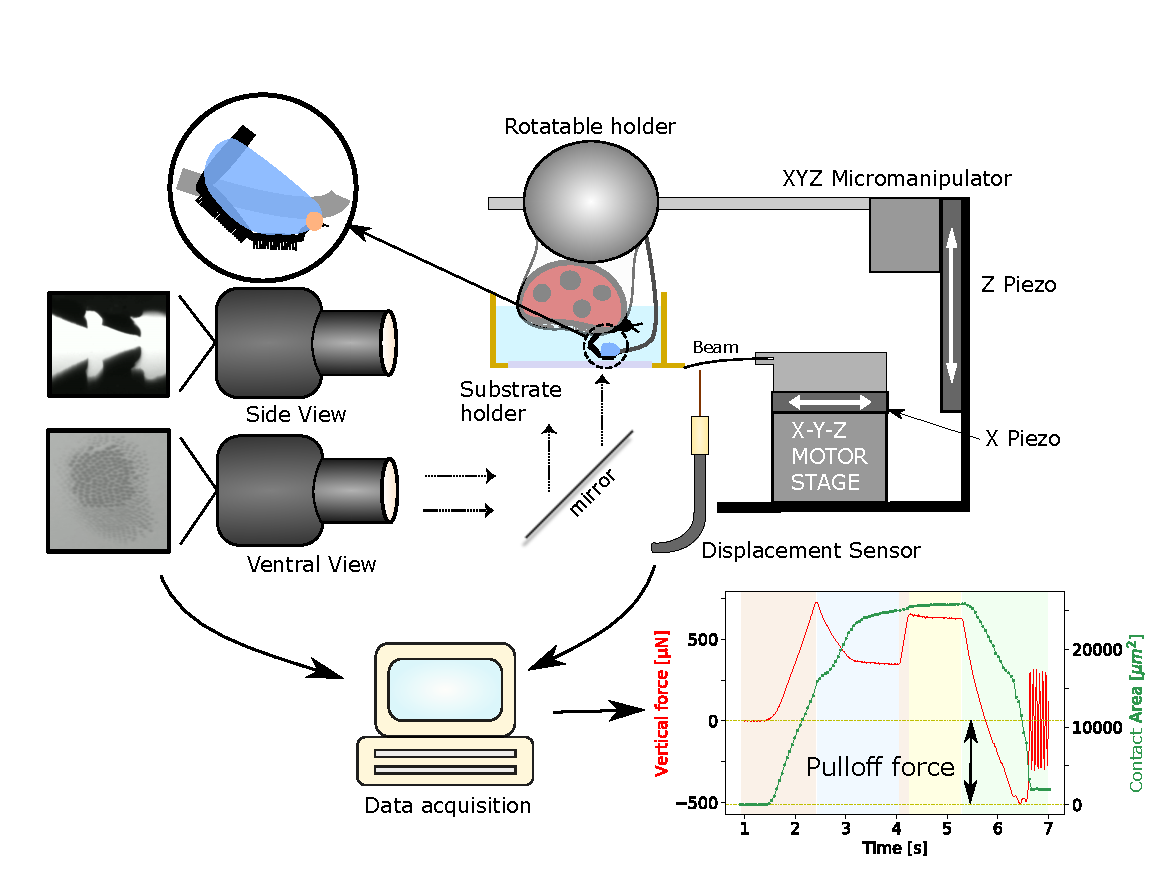
\includegraphics[width=6in]{Figure1-Setup_schematic}%
\caption[]{Adhesion test setup (see text for details). Top-left inset shows a magnified cartoon of the beetle's leg constrained to a solder wire (grey) using Blu Tack (blue) and epoxy glue (orange). The recorded force data and
contact area of a distal pad are shown in the bottom-right plot, in which, the shaded
regions from left to right represent the distinct movement sequence: approach, lateral pull, approach, pause and retract, respectively. Negative force values
represent attraction and the minimum force peak during the final retraction
step is the adhesion force used for further analysis. An animated version of a typical force recording is available in the supplementary material (see Movie1).}
\label{fig:Setup}
\end{figure*}


%\begin{figure}
%\begin{centering}
%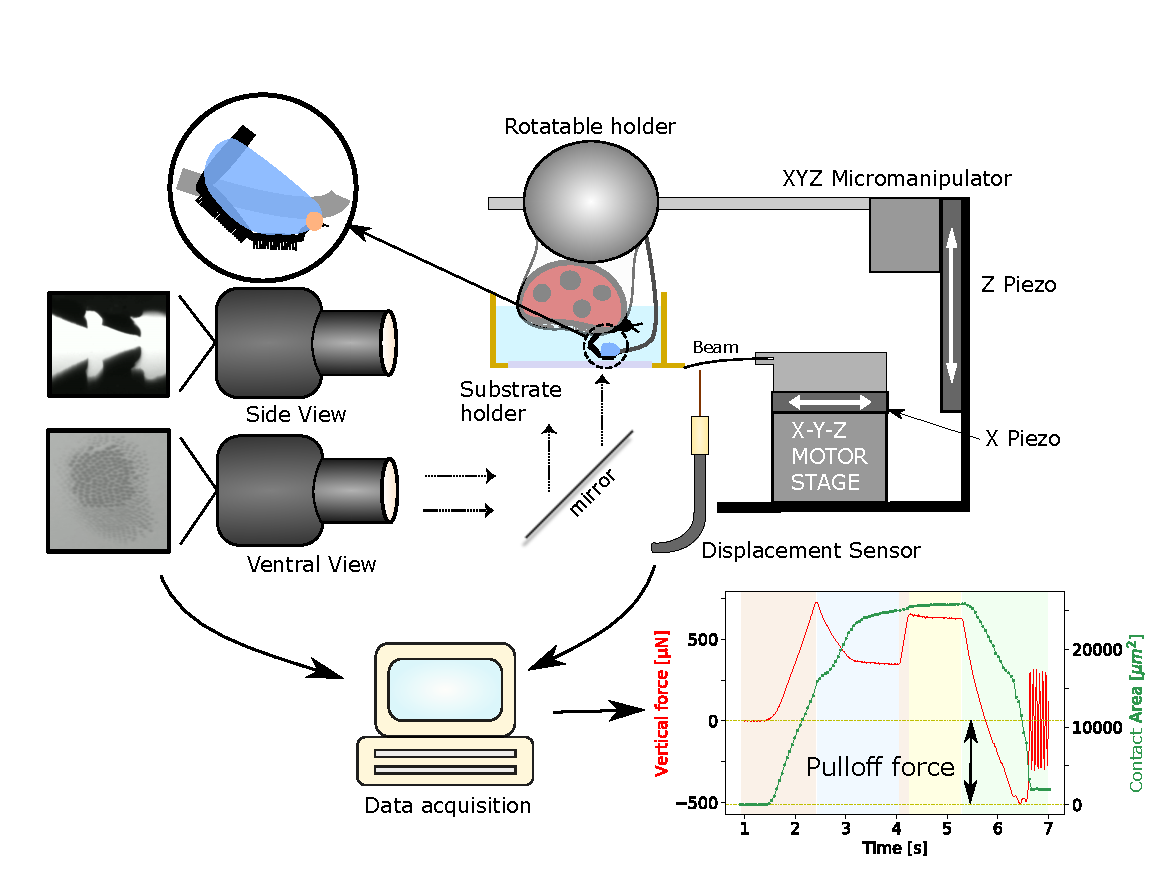
\includegraphics[width=3in]{Figure1-Setup_schematic}
%\par\end{centering}
%\caption{\label{fig:Setup} Adhesion test setup (see text for details). Top-left inset shows a magnified cartoon of the beetle's leg constrained to a solder wire (grey) using Blu Tack (blue) and epoxy glue (orange). The recorded force data and
%contact area of a distal pad are shown in the bottom-right plot, in which, the shaded
%regions from left to right represent the distinct movement sequence: approach, lateral pull, approach, pause and retract, respectively. Negative force values
%represent attraction and the minimum force peak during the final retraction
%step is the adhesion force used for further analysis. An animated version of a typical force recording is available in the supplementary material (see Movie1).}
%\end{figure}

\subsubsection{Data analysis}

Extraction of pull-off force from force data, image processing, plotting
and statistical analysis were all performed in ``\emph{Buggee}'',
a software tool written in Python using open-source libraries for synchronous
analysis of force data and video recordings (\url{https://github.com/PranavSudersan/Buggee}). 

For measurements in air, the pull-off force was defined as the minimum
negative force during the retraction step (bottom-right plot in Figure \ref{fig:Setup}).
For underwater measurements, an additional correction was necessary.
When the beetle was partially submerged underwater, its contact line at the
water surface shifted, which influenced the force readout due to surface
tension and buoyancy. This effect needed to be cancelled. Therefore, a ``background''
force data was recorded, where the submerged beetle makes no contact
with the substrate. This background data was then subtracted from
a typical force curve with substrate contact to correct for the external
surface tension effects. The pull-off force was subsequently calculated
from the minima as before. 

Data sets were compared for statistical differences using two-way ANOVA analysis, with \emph{contact mode} and \emph{substrate chemistry} as the categorical variables and \emph{adhesion force} as the dependant variable. Pairwise
Student t-test were done for post-hoc analysis and their corresponding p-value and Common Language
Effect Size (CLES) are reported. Shapiro-Wilk tests were done for each
data set to verify a normal distribution of its residuals and Levene's
test was done to check for variance homogeneity, to validate the ANOVA 
assumptions. Bonferroni's correction was used to account for multiple
comparison between groups.

\subsubsection{Substrate preparation}

Standard 20 mm wide glass cover-slips were used as the hydrophilic
substrate. Glass was wiped with isopropanol, rinsed in water and dried
under nitrogen flow before use. For the hydrophobic substrate, the glass cover slip was coated with
a fluorosilane via chemical vapour deposition (CVD). First, the glass
was cleaned using IPA. The surface was then plasma cleaned in an oxygen
plasma chamber (\emph{Femto, Diener Electronic GmbH, Germany}) for 10 min at 120 W. Next, 0.2 ml of
Trichloro(1H,1H,2H,2H-perfluorooctyl) silane (PFOTS), procured from
Sigma Aldrich, was put in a sealed chamber along with the the cleaned
glass. The chamber was placed under 100 mbar pressure for 10 min for
the CVD process. Finally, the substrate was annealed at 150 \textcelsius{}
for 3 hours. Henceforth, we refer to the hydrophilic untreated glass substrate 
as simply \emph{Glass} and the hydrophobic fluorinated glass substrate as \emph{PFOTS}.

The surface chemistry was characterised by dynamic contact angle
measurements, performed with a contact angle goniometer (\emph{OCA 35, DataPhysics Instruments GmbH, Germany}).
The substrate's wetting towards a polar (Milli-Q water) and a non-polar (n-hexadecane) liquid was tested. Advancing
and receding contact angles were measured for a maximum drop volume
of 10 \textmu l and with 0.5 \textmu l s\protect\textsuperscript{-1} flow rate (see supplementary section S2).

\subsection{Results}

%\subsubsection{Adhesion measurements}

In air, adhesion forces of the distal pad of the ladybug beetles against
glass and PFOTS were similar, i.e. no significant differences were
detected (Figure \ref{fig:Effect-of-contact} and supplementary section S3).
In contrast, the underwater adhesion on a PFOTS surface was significantly
larger than on glass (p < 0.001). This stronger adhesion on PFOTS
was observed both in the presence and absence of a trapped bubble.
In both cases, the adhesion force reached similar values as in air. In contrast,
on glass, adhesion underwater was significantly reduced when compared
to dry conditions, irrespective of the presence of a trapped bubble
(p $\leq$ 0.002). In the presence of a bubble, underwater adhesion on glass was slightly higher (CLES = 0.84, p = 0.07).

\begin{figure}
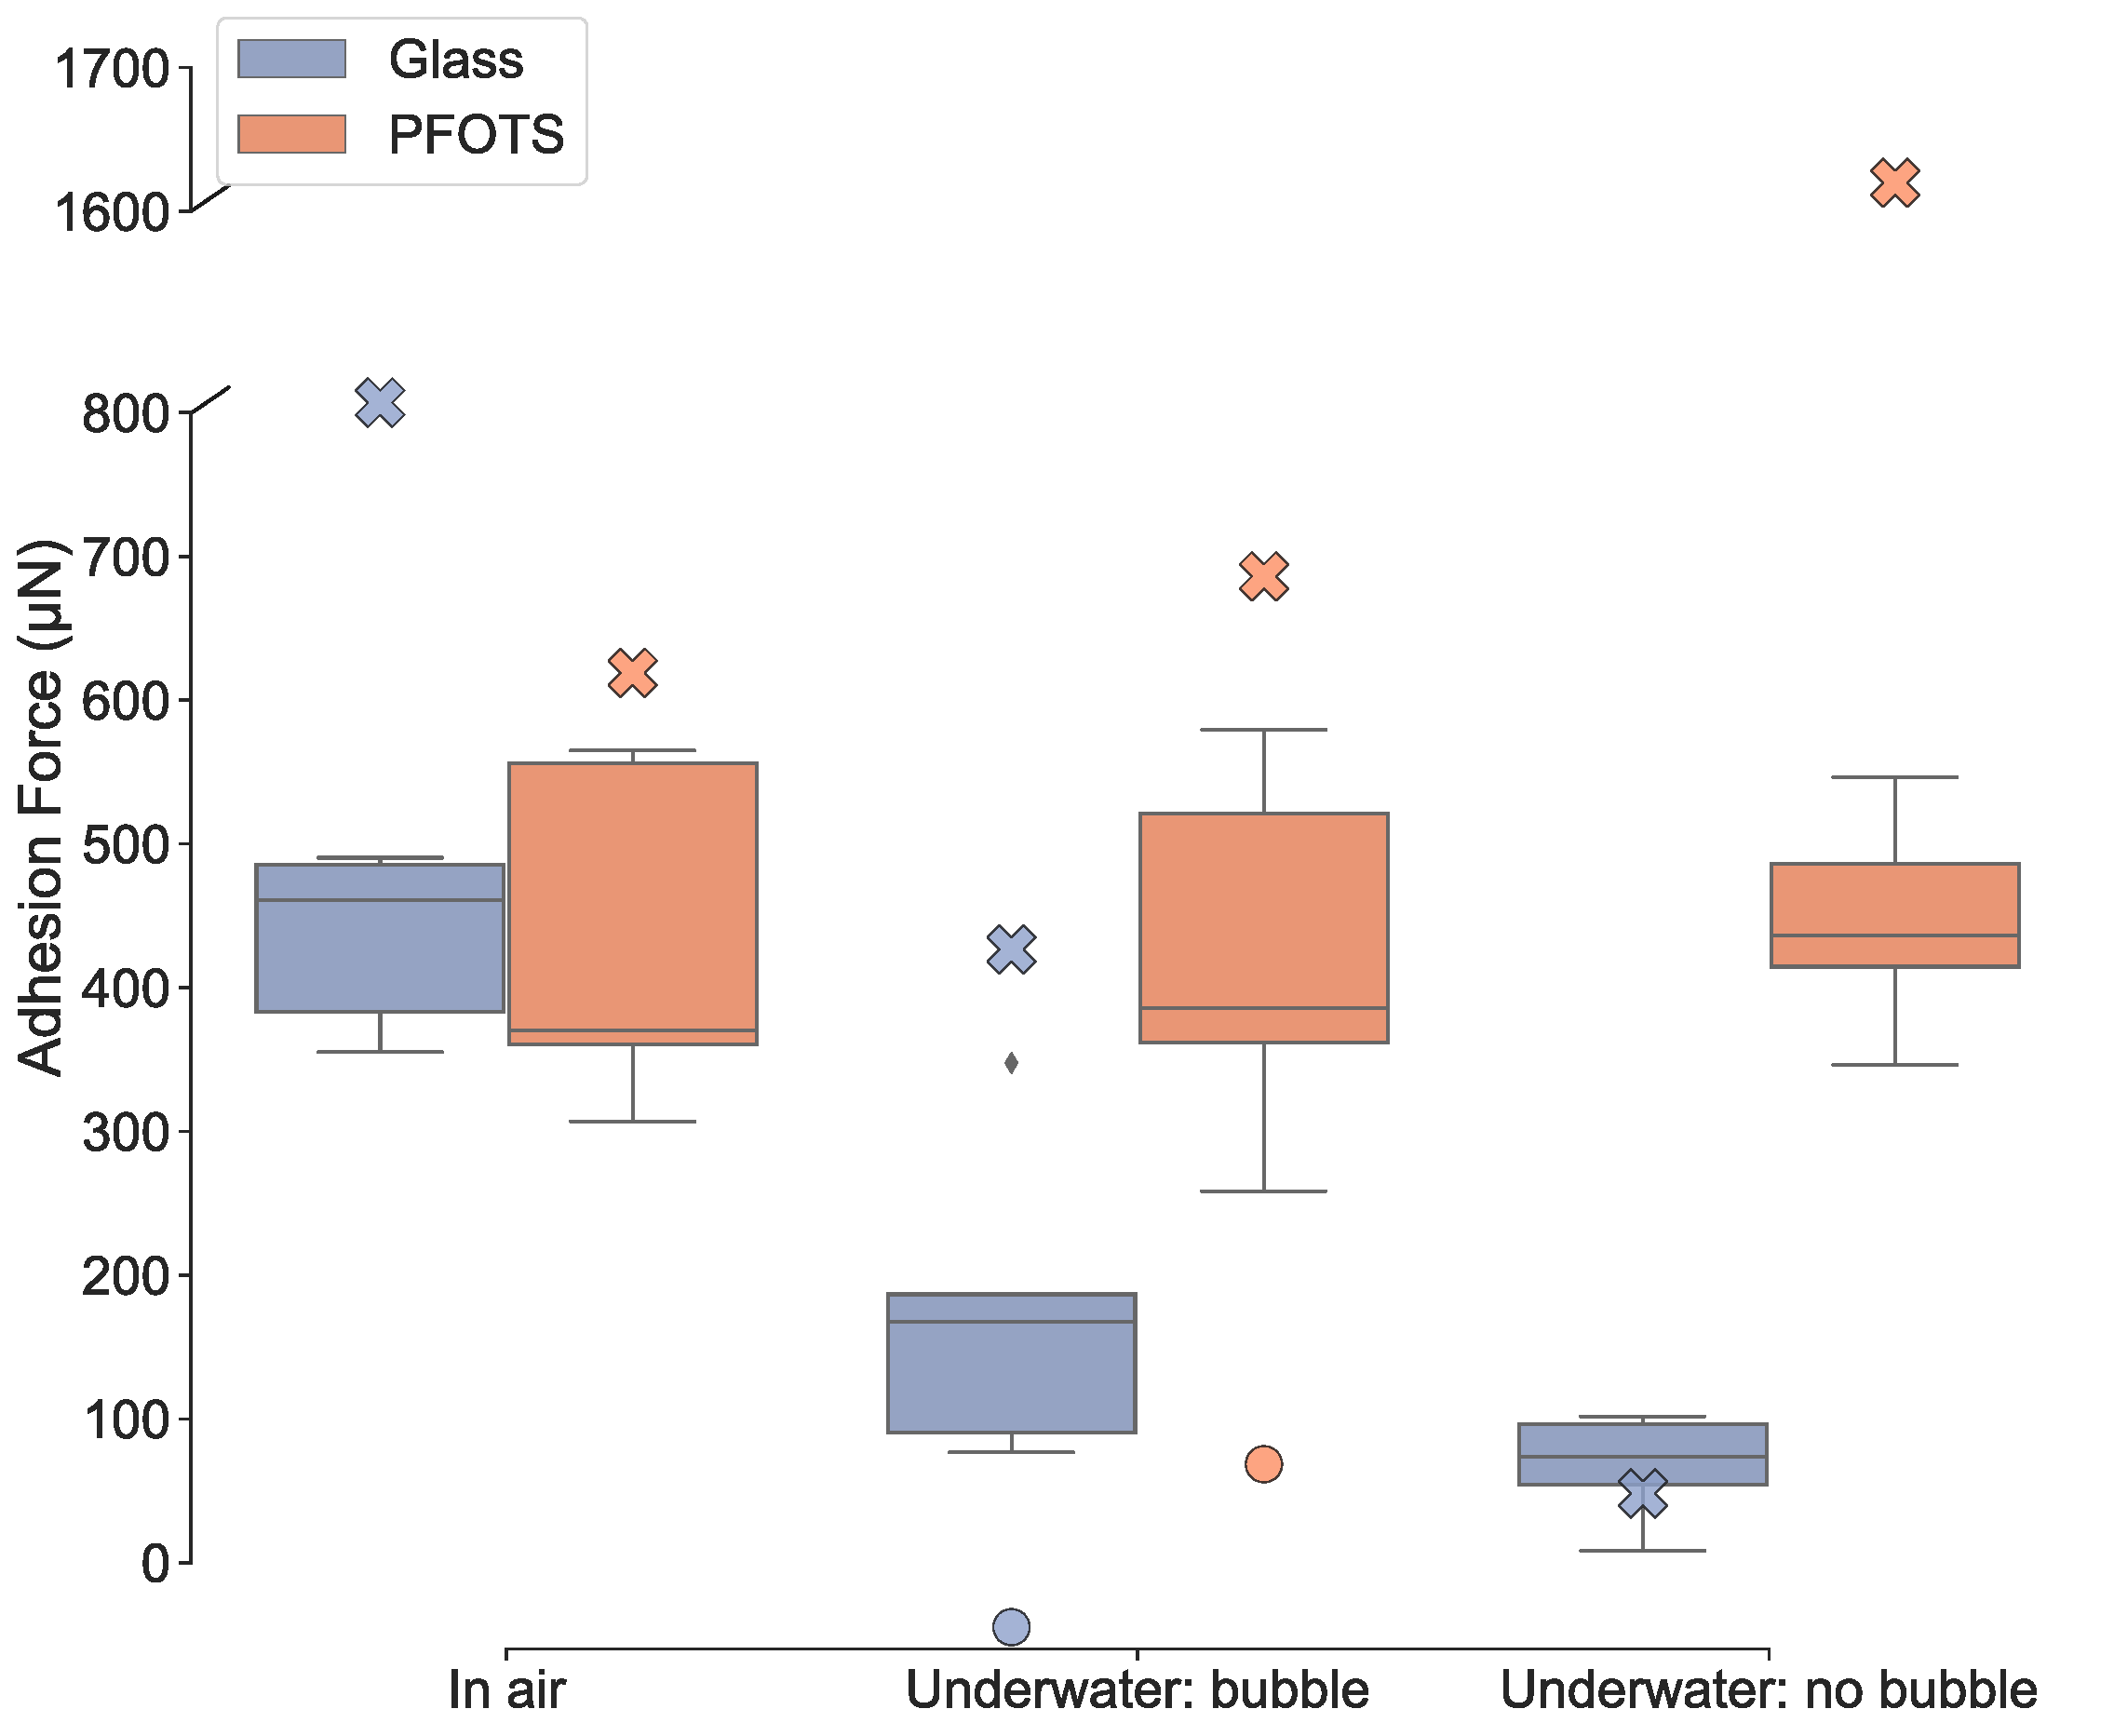
\includegraphics[width=3.5in]{Figure2-Expt_effect_of_contact}\caption{\label{fig:Effect-of-contact}Box-and-whisker plot showing
 adhesion force measurements of ladybug beetle's (\emph{Coccinella
septempuctata}) distal pad on untreated hydrophilic glass (blue) and hydrophobic PFOTS coated glass (red) substrates in air and underwater
conditions (n=5 per box). The two modes of contact during underwater experiments
are represented separately: \textquotedblleft\emph{bubble}\textquotedblright{}
and \textquotedblleft\emph{no bubble}\textquotedblright . The small diamonds represent outlier points. Crosses
represent theoretical predictions of adhesion force, while, circles
represent the contribution of the bubble itself, calculated from the
capillary bridge model (see text). In the model, hair diameter = 4 \textmu m,
pad diameter = 200 \textmu m, hair length = 40 \textmu m,
N\protect\textsubscript{hairs} = 500, V\protect\textsubscript{fluid}
= 4.2 fL and V\protect\textsubscript{bubble} = 1.2 nL. Interfacial
tension of the tarsal adhesive fluid in air and water were assumed to be
24 mN m\protect\textsuperscript{-1} and 48 mN m\protect\textsuperscript{-1} respectively and water surface tension is 72 mN m\protect\textsuperscript{-1}.}
\end{figure}

Apart from the three depicted contact modes, we observed an additional
fourth mode which occurred in roughly 25\% of our underwater experiments using degassed water.
In this scenario, the ventral view recordings show that none of the hairs
appear to contact well with either glass or PFOTS substrate (supplementary data: Movie2), unlike the other
three contact modes (supplementary data: Movie1). This ``bad contact'' scenario only happened underwater and shows no adhesion 
with either glass or PFOTS substrate. While it was not completely
clear why such a contact occurs, there can be two possible reasons.
First, the hairs could get bundled due to a small air bubble trapped within
them which might not have completely dissolved away in the water.
The presence of this air-water meniscus could thus lead to elasto-capillary bundling of the hairs, resulting in their disorientation. Second, a thin water
layer at the substrate interface might not be drained out to allow
the hairs to make contact with the substrate, resulting in a loss
of adhesion.


\section{Theory}

\subsection{Capillary Bridge Model}

We modelled the hairy pad as an array of $N$ cylindrical rods of length,
$L$, and diameter, $D_{h}$, fixed to a flat circular pad of diameter,
$D_{p}$ (Figure \ref{fig:Model}). The hairs and the pad were assumed
to be perfectly rigid, for simplicity. The tip of each hair has a tarsal 
adhesive fluid of volume $V_{f}$, mediating contact with the substrate.
The fluid is pinned to the circumference of the hair and forms a capillary
bridge of height, $d$. Similar to our experiments, we considered three
modes of contact for the pad: 1) \emph{In air}, 2) \emph{Underwater:
no bubble} and 3) \emph{Underwater: bubble}. In the third case, a
bubble of volume, $V_{b}$, is trapped between the hairs and pinned
to the pad circumference.

\begin{figure}
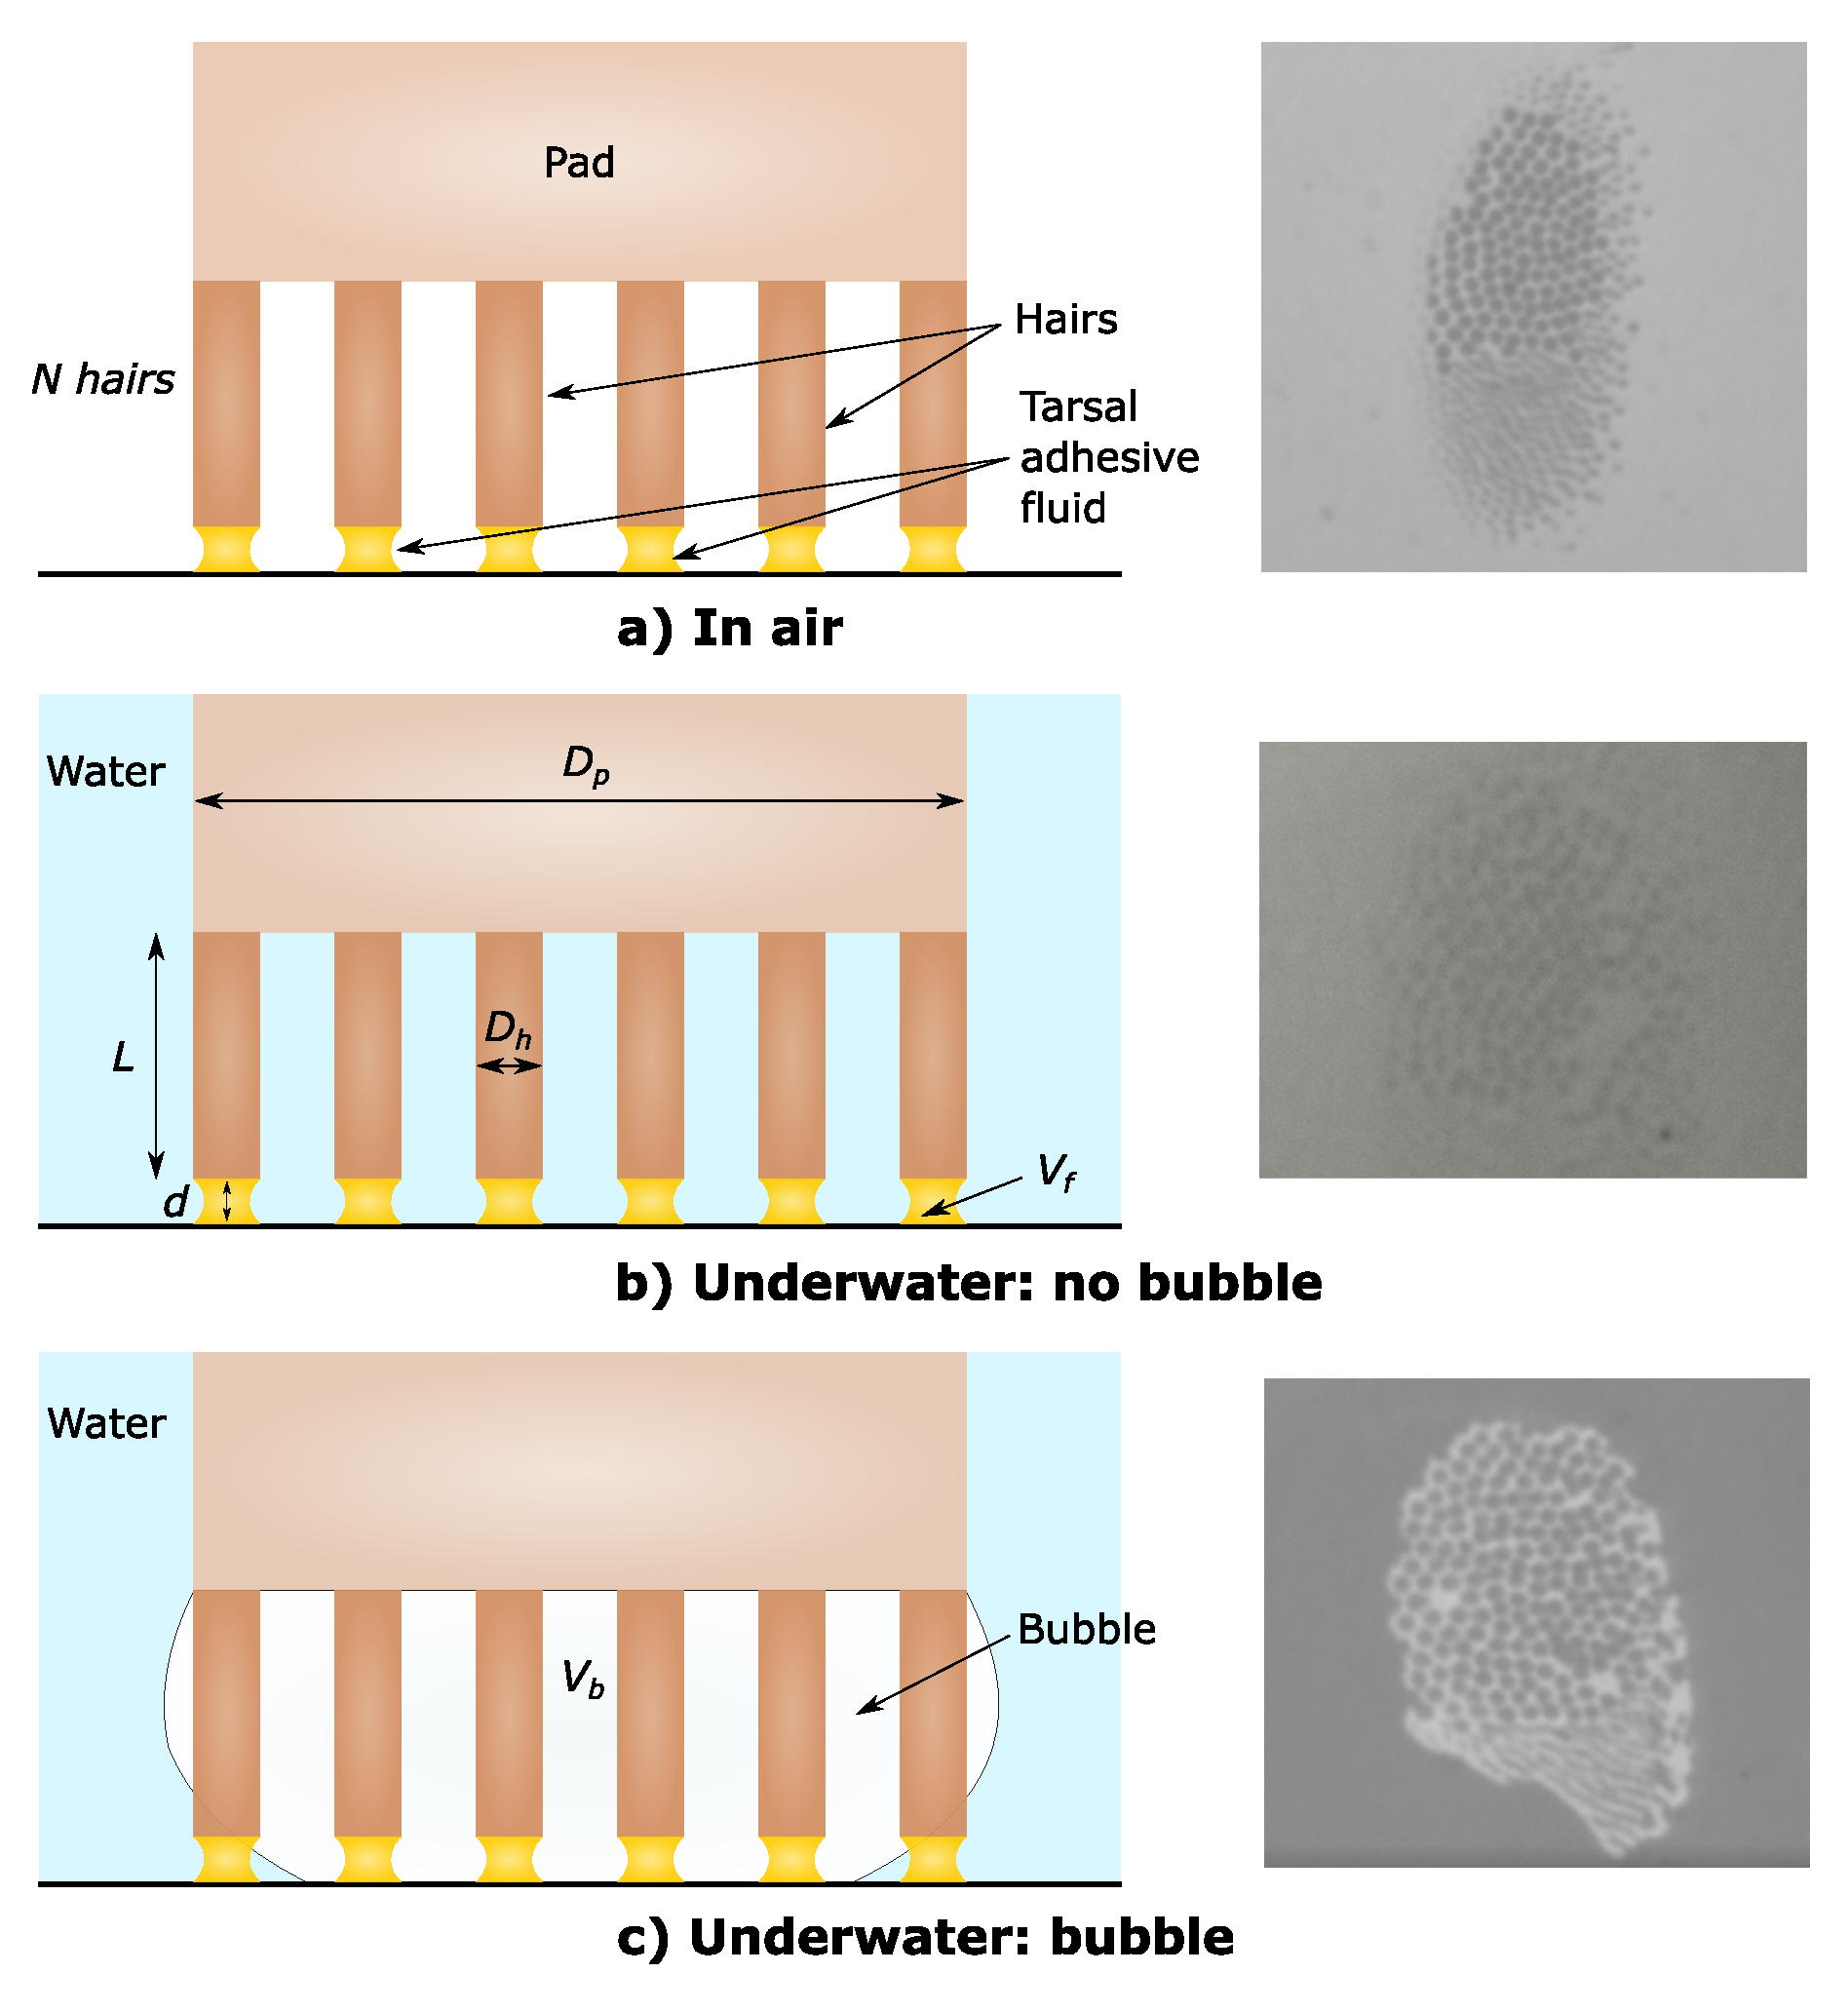
\includegraphics[width=3.5in]{Figure3-Model_schematic}
\caption{\label{fig:Model}The capillary bridge model of a hairy adhesive pad. The hairs make contact
with the substrate (hydrophilic or hydrophobic) in three modes: a) \emph{In air}, where the tarsal adhesive
fluid bridges are surrounded by air; b) \emph{Underwater: no bubble},
where the fluid bridges are fully surrounded by water; c)\emph{
Underwater: bubble}, where part of the fluid bridges are
inside the bubble while others are outside in water (see text for details). The corresponding
ventral view contact images of the beetle's pad seen during adhesion experiments are shown on the right.}
\end{figure}

To characterise the tarsal adhesive fluid and bubble volume, we defined two
radii, $s_{f}$ and $s_{b}$, respectively, by $V_{f}=\frac{4}{3}\pi s_{f}^{3}$
and $V_{b}=\frac{4}{3}\pi s_{b}^{3}$. Here, $s_{f}$ and $s_{b}$
are the radii of spheres with equivalent volumes. Fluid and bubble
radii were assumed to scale proportional to their corresponding pinned
contact diameter. We thus defined the size parameters, $\phi_{f}=D_{h}/(2s_{f})$
and $\phi_{b}=D_{p}/(2s_{b})$ for the fluid and bubble
respectively, to conveniently scale their volumes relative to the
hair and pad diameters they are pinned to.

The net force for cases 1 and 2 can be calculated as:

\begin{equation}
F_{net}=Nf\label{eq:f_air/water}
\end{equation}

Here, $f$ is the capillary force of a single fluid bridge at a distance,
$d$, in air ($f_{air}$) or underwater ($f_{water}$).

For case 3, the net force is given by:

\begin{equation}
F_{net}=N_{in}f_{air}+N_{out}f_{water}+f_{bubble}\label{eq:f_bubble}
\end{equation}

Here, $N_{in}$ and $N_{out}$ are the number of hairs inside and
outside the bubble, respectively, $f_{air}$ and $f_{water}$ are
the capillary forces of the fluid bridge inside and outside the bubble,
respectively, and $f_{bubble}$ is the capillary force contribution
due to the bubble meniscus alone at distance $d+L$. 

The capillary force, $f$, is the sum of two contributions: Laplace pressure and  surface
tension, as given by:
\begin{equation}
f=\varDelta P_{laplace}A_{_{bottom}}+2\pi R_{bottom}\gamma\sin\theta\label{eq:f_bridge}
\end{equation}

Here, $\varDelta P_{laplace}$ is the Laplace pressure of the equilibrium
capillary bridge, $\theta$ is the contact angle, $A_{bottom}$ is the contact area of the capillary
bridge with the substrate at bottom and $R_{bottom}$ is the corresponding
radius of contact. Unlike previous analytical treatments \citep{RN203, RN318}, force versus distance for a single capillary bridge was calculated by Surface
Evolver simulations \citep{RN206, RN93},
and used to obtain $F_{net}$ as a function of $d$ for each mode
of contact  (see supplementary section S1 for details). The adhesion force of the complete hairy pad system was
then obtained from the minima of $F_{net}$, where negative force
values represent attraction.

We considered $f_{air}$ and $f_{water}$ to be distinct terms
because the capillary force by the tarsal adhesive fluid would be different
in air and underwater due to its different contact angle and interfacial
tension in each case. Using the Young-Dupr\'{e} equations
for each case of fluid-air, fluid-water and water-air interface, one
can derive the following relation for the contact angle of the tarsal adhesive
fluid underwater:

\begin{equation}
\cos\theta_{fw}=\frac{\gamma_{fa}\cos\theta_{fa}-\gamma_{wa}\cos\theta_{wa}}{\gamma_{fw}}\label{eq:theta_fw}
\end{equation}

Here, $\theta_{fw}$ and $\theta_{fa}$ are the contact angles of
the tarsal adhesive fluid with the substrate in water and air respectively,
$\theta_{wa}$ is the contact angle of water with the substrate in
air, $\gamma_{fa}$ is the surface tension of the tarsal adhesive fluid,
$\gamma_{wa}$ is the surface tension of water and $\gamma_{fw}$
is the interfacial tension of the tarsal adhesive fluid with water.
%
%All lengths ($D_{h}$, $D_{p}$, $L$, $d$) were normalised w.r.t. $s_{f}$ and forces were normalized
%w.r.t. $\gamma_{fa}s_{f}$. Interfacial tension values were fixed relative
%to $\gamma_{fa}$. Non dimensional bubble volume was expressed as,
%$\hat{V}_{b}=V_{b}/s_{f}^{3}$

Geometric parameters and interfacial properties were kept fixed for
all model calculations (Table \ref{tab:Model-parameters}). Here,
we assumed the tarsal adhesive fluid to have similar interfacial tension values as n-hexadecane \citep{RN320}. Experimental receding contact angle values for n-hexadecane and water
on untreated (hydrophilic) and fluorinated (hydrophobic) glass surface were used as 
 $\theta_{fa}$ and $\theta_{wa}$, respectively (Table S1).
Hair and pad geometry, and tarsal fluid volume were assumed to be values typical
for a ladybug's hairy pad \citep{RN19, RN108}.

First, we calculated force-distance curves for a single pinned liquid
capillary bridge. Second, the effect of substrate on the force-distance
curves of the hairy pad system was compared for each mode of contact.
Third, we looked at the effect of changing the bubble
volume, $\hat{V}_{b}$, on the net underwater adhesion.
Finally, the influence of varying the hair diameter, $D_{h}$, on adhesion
was studied for each case.

%\begin{table}
%\centering{}%
%\begin{tabular}{|l|c|}
%\hline 
%Property & Value\tabularnewline
%\hline 
%\hline 
%Contact area fraction, $\alpha$ & 0.1\tabularnewline
%\hline 
%Hair aspect ratio, $L/D_{h}$ & 10\tabularnewline
%\hline 
%Water surface tension ratio, $\gamma_{wa}/\gamma_{fa}$ & 3\tabularnewline
%\hline 
%Tarsal fluid-water interfacial tension ratio, $\gamma_{fw}/\gamma_{fa}$ & 2\tabularnewline
%\hline 
%Tarsal fluid size parameter, $\phi_{f}$ & 2\tabularnewline
%\hline 
%Hydrophilic substrate & $\theta_{fa}=6\lyxmathsym{\textdegree}$, $\theta_{wa}=24\lyxmathsym{\textdegree}$\tabularnewline
%\hline 
%Hydrophobic substrate & $\theta_{fa}=50\lyxmathsym{\textdegree}$, $\theta_{wa}=120\lyxmathsym{\textdegree}$\tabularnewline
%\hline 
%\end{tabular}\caption{\label{tab:Model-parameters}Fixed parameter values corresponding to the pad's geometry, 
%tarsal fluid and substrate wetting properties used in the capillary bridge model}
%\end{table}

%\begin{table}[!t]
%\processtable{Fixed parameters corresponding to the pad's geometry, 
%tarsal fluid and substrate wetting properties used in the capillary bridge model \label{tab:Model-parameters}}
%{\begin{tabular*}{3.5in}{@{\extracolsep{\fill}}lllll@{}}
%\hline
%\TCH{Property} & \TCH{Value} \\
%\hline
%Contact area fraction, $\alpha$ & 0.1\\
%Hair aspect ratio, $L/D_{h}$ & 10\\
%Water surface tension ratio, $\gamma_{wa}/\gamma_{fa}$ & 3\\
%Tarsal fluid-water interfacial tension ratio, $\gamma_{fw}/\gamma_{fa}$ & 2\\
%Tarsal fluid size parameter, $\phi_{f}$ & 2\\
%\multirow{2}{*}{Hydrophilic substrate wetting} &  $\theta_{fa}=6\lyxmathsym{\textdegree}$\\
%    & $\theta_{wa}=24\lyxmathsym{\textdegree}$\\
%\multirow{2}{*}{Hydrophobic substrate wetting} &  $\theta_{fa}=50\lyxmathsym{\textdegree}$\\
%    & $\theta_{wa}=120\lyxmathsym{\textdegree}$
%\end{tabular*}}{}
%\end{table}

\begin{table}[!t]
\processtable{Fixed parameters corresponding to the pad's geometry, 
tarsal fluid and substrate wetting properties used in the capillary bridge model \label{tab:Model-parameters}}
{\begin{tabular*}{3.5in}{@{\extracolsep{\fill}}lllll@{}}
\hline
\TCH{Property} & \TCH{Value} \\
\hline
Number of hairs, $N$ & 500\\
Hair diameter, $D_{h}$ & 4 \textmu m\\
Pad diameter, $D_{p}$ & 200 \textmu m\\
Hair length, $L_{h}$ & 40 \textmu m\\
Water surface tension, $\gamma_{wa}$ & 72 mN m\textsuperscript{-1}\\
Tarsal fluid-air surface tension, $\gamma_{fw}$ & 27 mN m\textsuperscript{-1}\\
Tarsal fluid-water interfacial tension, $\gamma_{fw}$ & 55 mN m\textsuperscript{-1}\\
Tarsal fluid volume, $V_{f}$ & 4 fL\\
Bubble volume, $V_{b}$ & 1 nL\\
\multirow{2}{*}{Hydrophilic substrate wetting} &  $\theta_{fa}=6\lyxmathsym{\textdegree}$\\
    & $\theta_{wa}=20\lyxmathsym{\textdegree}$\\
\multirow{2}{*}{Hydrophobic substrate wetting} &  $\theta_{fa}=56\lyxmathsym{\textdegree}$\\
    & $\theta_{wa}=93\lyxmathsym{\textdegree}$
\end{tabular*}}{}
\end{table}

\subsection{Capillary force of a single liquid bridge\label{subsec:Capillary-force-of}}

Forces due to a single pinned capillary liquid bridge in contact with
a substrate were obtained via Surface Evolver simulations (Figure \ref{fig:Single-bridge}).
We see that, generally, the shape of the liquid meniscus determines
the strength of its adhesion force. High adhesion is seen for contact
angles less than $\sim$ 70\textdegree{} due to a net negative (convex) curvature
of the meniscus, while low adhesion is seen for contact angles greater
than $\sim$ 150\textdegree{} due to its net curvature being close
to zero. The Laplace pressure contribution to the net adhesion force
dominates for contact angles less than 100\textdegree{} (Figure \ref{fig:Single-bridge}b).
Interestingly, its contribution to the adhesion force is mostly non-repulsive
for contact angles greater than 90\textdegree . This is because, the
low volume of the liquid and its pinned contact line prevents the
meniscus from having a high positive (concave) curvature due to geometric constraints.
Only for a contact angle of 150\textdegree , the liquid's curvature
becomes positive, manifested in its slightly repulsive Laplace contribution.
Surface tension makes a significant contribution to the net force
only for a small range of contact angles close to 90\textdegree .
For contact angles greater than 150\textdegree , the net adhesion
force approaches zero.


\begin{figure*}[!t]
\centering
\subfloat[Force-distance curves]{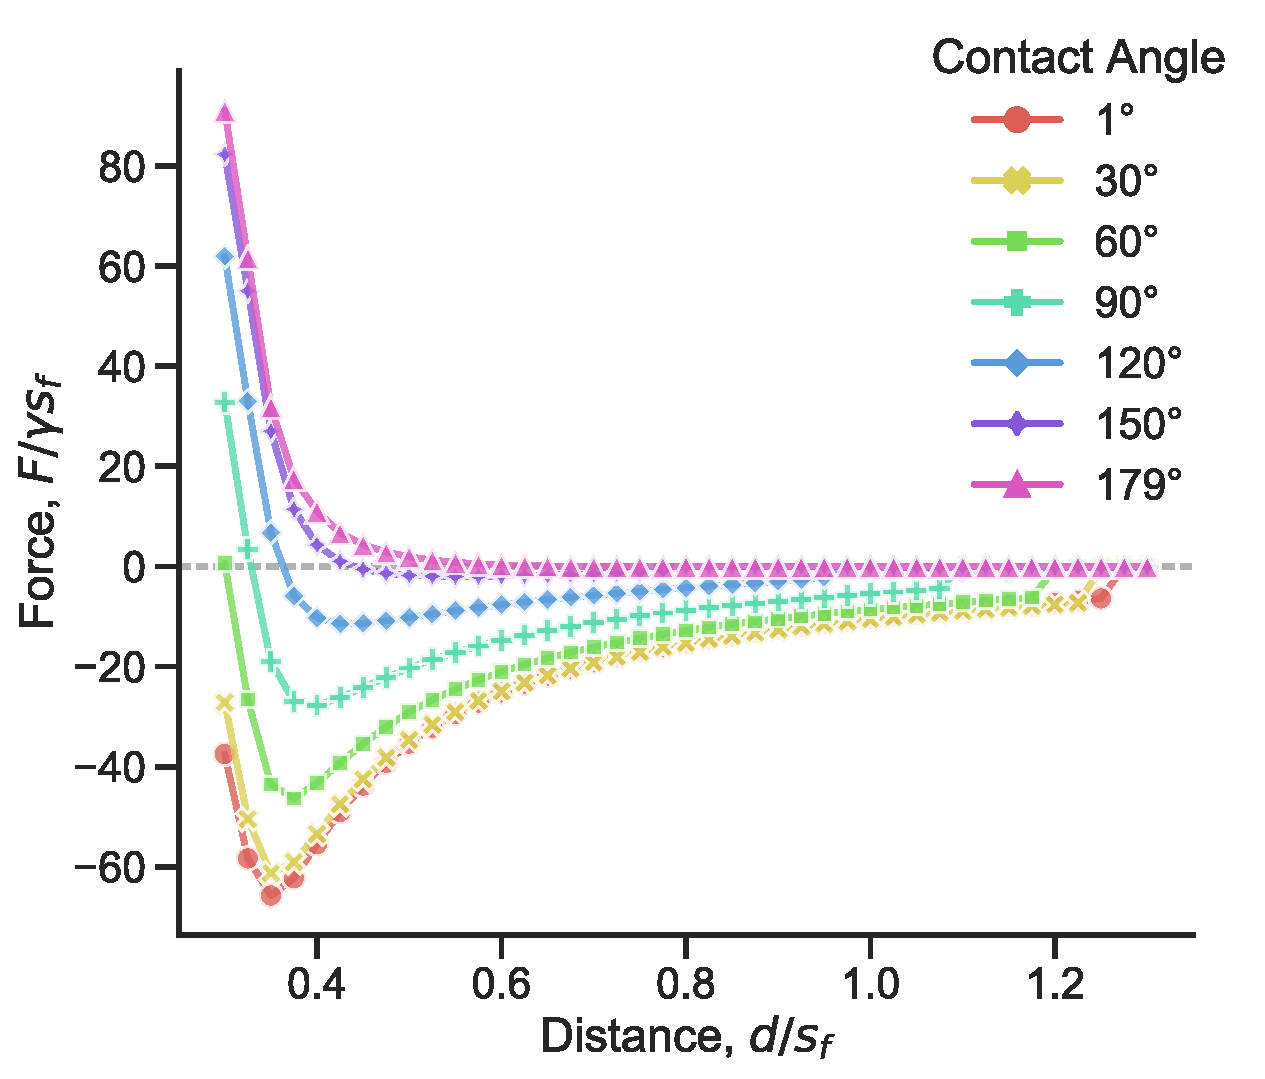
\includegraphics[width=3in]{Figure4a-Single_bridge_fd}\label{fig_first_case}}%
\hskip3pc
\subfloat[Force contributions]{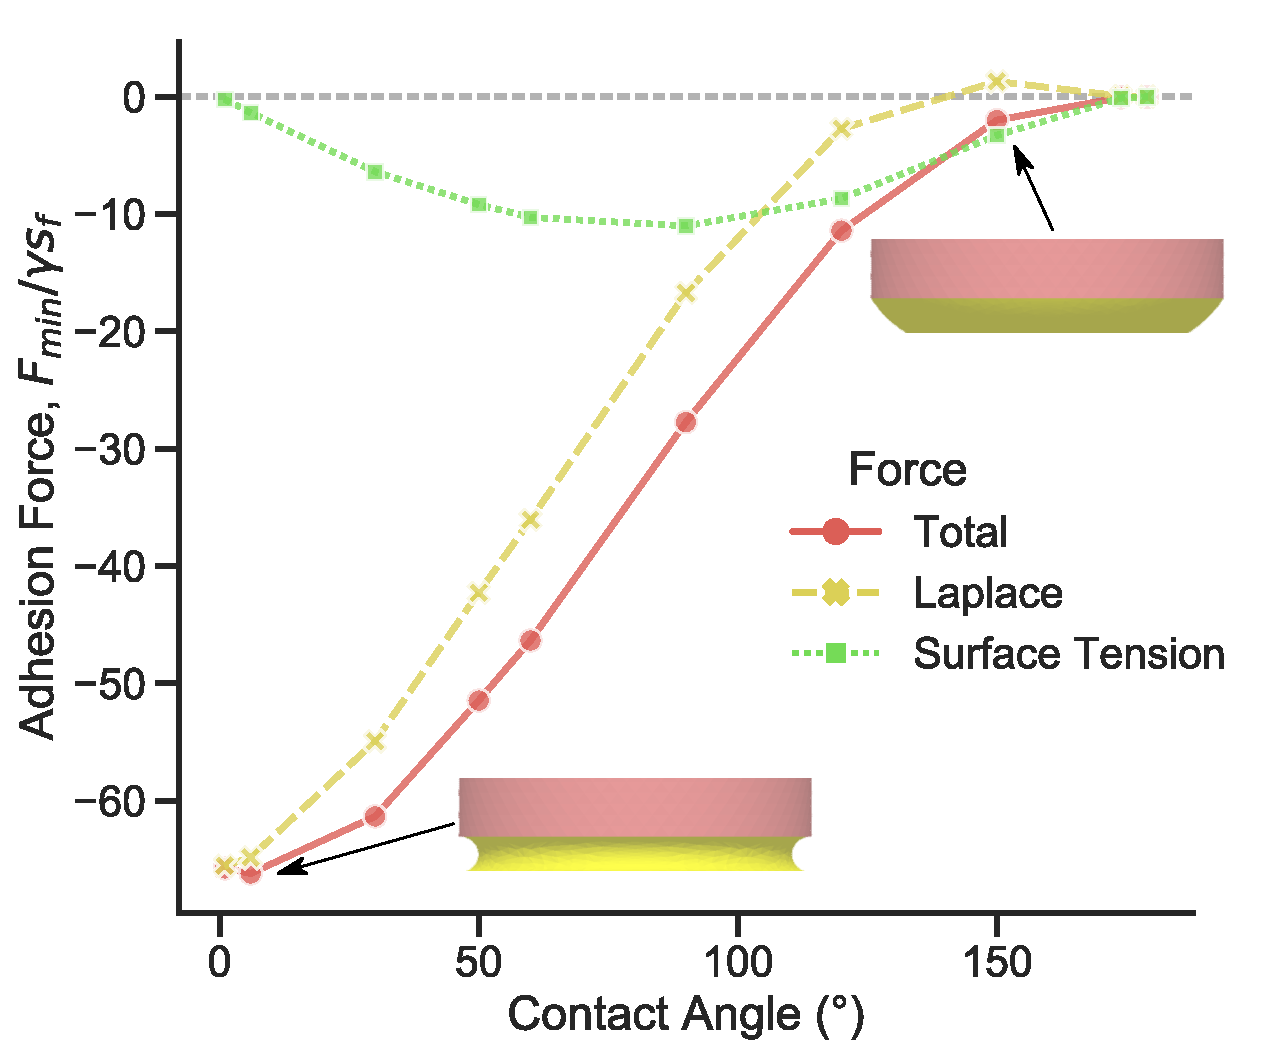
\includegraphics[width=3in]{Figure4b-Single_bridge_force_contribution}\label{fig_second_case}}%
\caption[]{Simulation of normalised capillary force of a single liquid
bridge in contact with a substrate and pinned to a circular perimeter
on top. Fluid size parameter, $\phi_{f}=2$. Negative force values
represents attraction. a) Force-distance curves are shown for different
contact angles of the liquid with the substrate. b) Adhesion forces,
calculated from the minima of the corresponding force-distance curves,
are plotted as a function of contact angle with the substrate, together
with its Laplace and surface tension components (equation S1 in supplementary section).
Simulation snapshots of the liquid meniscus corresponding to angles
6\textdegree{} and 150\textdegree{} are depicted.}
\label{fig:Single-bridge}
\end{figure*}

%\begin{figure}
%%\begin{minipage}[t]{0.5\columnwidth}%
%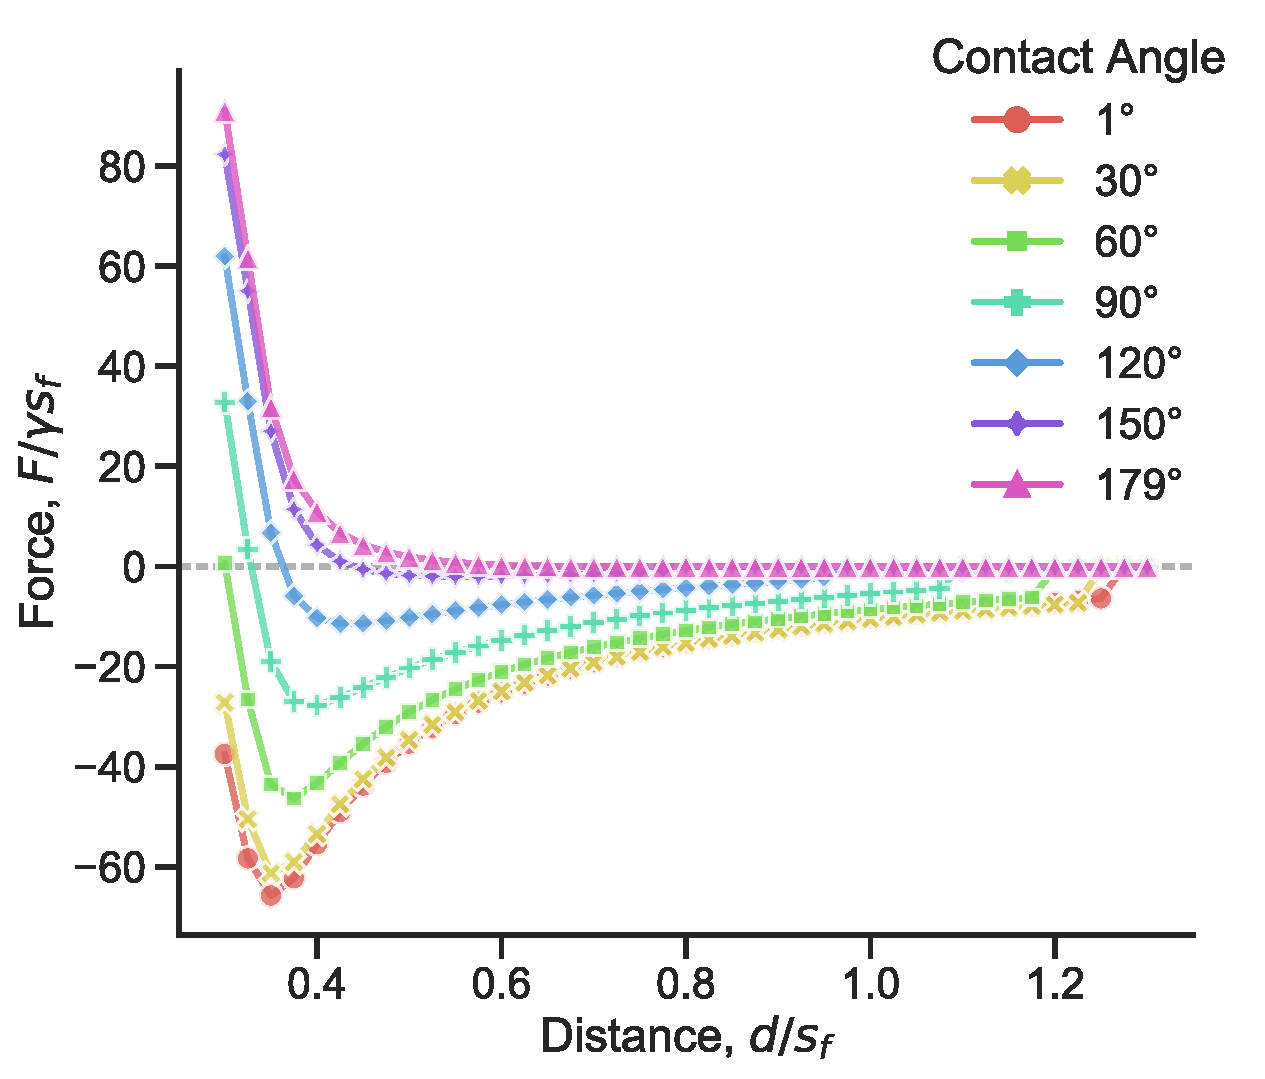
\includegraphics[scale=0.5]{Figure4a-Single_bridge_fd}
%
%\subcaption{Force-distance curves}%
%\end{minipage}\hfill{}%
%\begin{minipage}[t]{0.5\columnwidth}%
%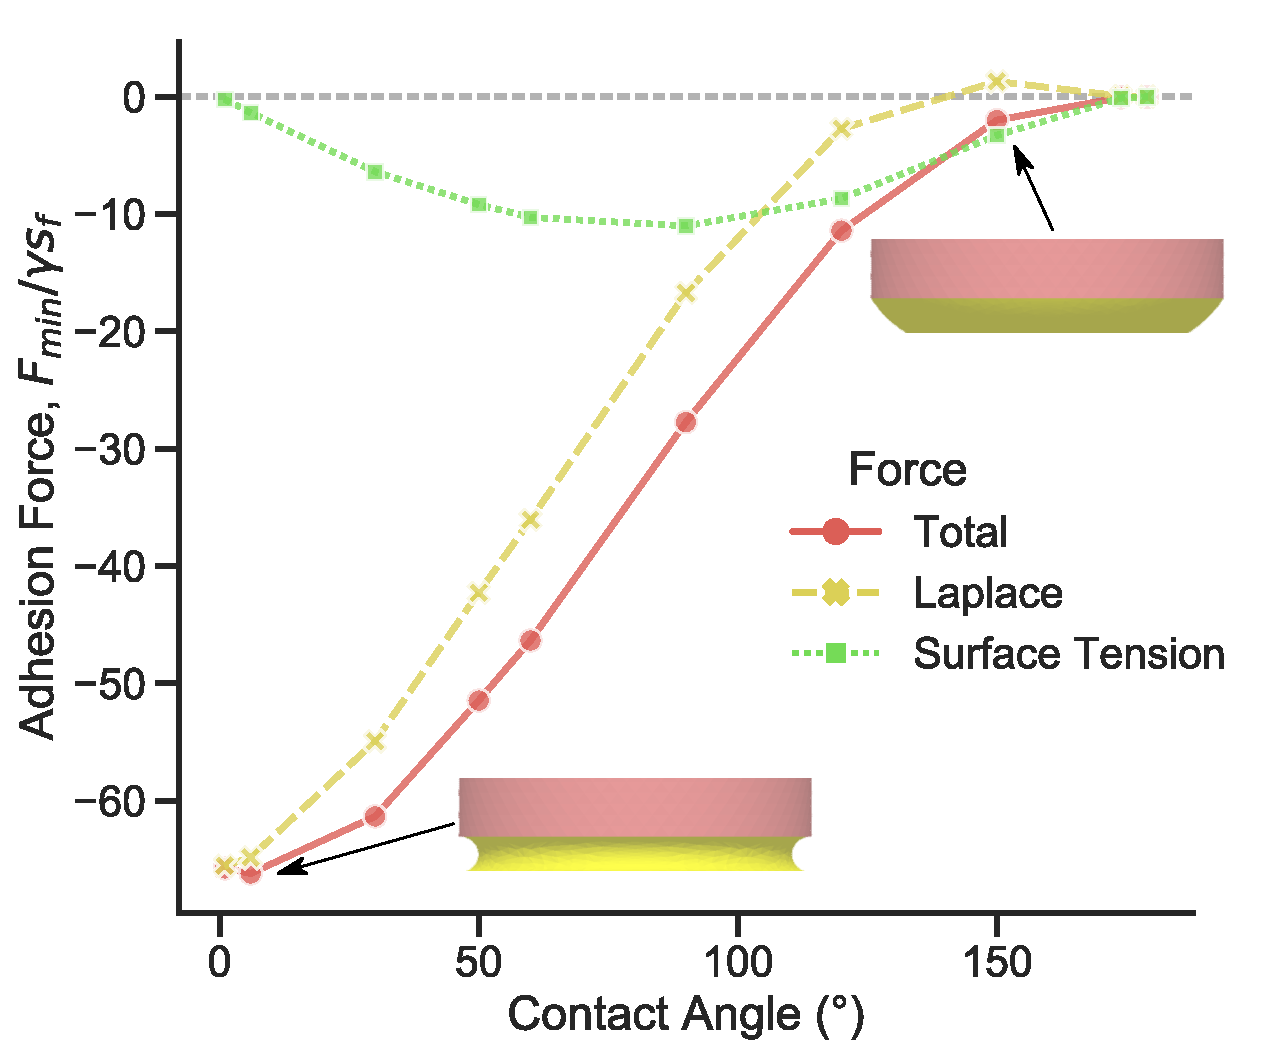
\includegraphics[scale=0.5]{Figure4b-Single_bridge_force_contribution}
%
%\subcaption{Force contributions}%
%\end{minipage}
%\caption{\label{fig:Single-bridge}Simulation of normalised capillary force of a single liquid
%bridge in contact with a substrate and pinned to a circular perimeter
%on top. Fluid size parameter, $\phi_{f}=2$. Negative force values
%represents attraction. a) Force-distance curves are shown for different
%contact angles of the liquid with the substrate. b) Adhesion forces,
%calculated from the minima of the corresponding force-distance curves,
%are plotted as a function of contact angle with the substrate, together
%with its Laplace and surface tension components (equation S1 in supplementary section).
%Simulation snapshots of the liquid meniscus corresponding to angles
%6\textdegree{} and 150\textdegree{} are depicted.}
%\end{figure}

The force-distance curves show a general trend of repulsive forces
at small distances (Figure \ref{fig:Single-bridge}a). This is a result
of the pinned contact line on the top. A limited volume is available
for the liquid to occupy when the gap distance is small, causing the
meniscus shape to bulge outwards near the pinned contact line. This
creates a net positive curvature, resulting in a positive Laplace
pressure and thus repulsion. Without pinning, the capillary forces
would have shown high attractive forces on a hydrophilic substrate\citep{RN93}. 
It is reasonable to expect the contact line to be mechanically pinned around the rim of the discoidal-shaped hair tip.
Since the male ladybug's pads are majorly composed of discoidal hairs, we proceed with this assumption to estimate the net adhesion
force of the whole pad.
%CHECK EVERYWHERE SHOULD BE DIMENSIONAL!
\subsection{Adhesion of a hairy pad: Effect of the substrate\label{subsec:Capillary-Bridge-Model:}}

The normalised force-distance curves of a hairy pad system on a hydrophilic
and hydrophobic substrate are predicted based on the capillary bridge
model and compared for the different contact modes (Figure \ref{fig:Effect-of-substrate}).
The forces in each case are calculated from equations (\ref{eq:f_air/water})
and (\ref{eq:f_bubble}) for fixed geometric and interfacial properties
(Table \ref{tab:Model-parameters}). 

On the hydrophilic substrate ($\theta_{wa}=24\lyxmathsym{\textdegree}$),
highest adhesion is seen when the hairs contact in air, while lowest
adhesion occurs underwater without a trapped bubble. The presence
of a bubble leads to intermediate force values. In contrast, on a
hydrophobic substrate ($\theta_{wa}=120\lyxmathsym{\textdegree}$),
highest adhesion is seen for the underwater case without a trapped
bubble, much larger than in air. When a bubble is present, the forces
are only slightly larger than in air. 

\begin{figure*}
\centering
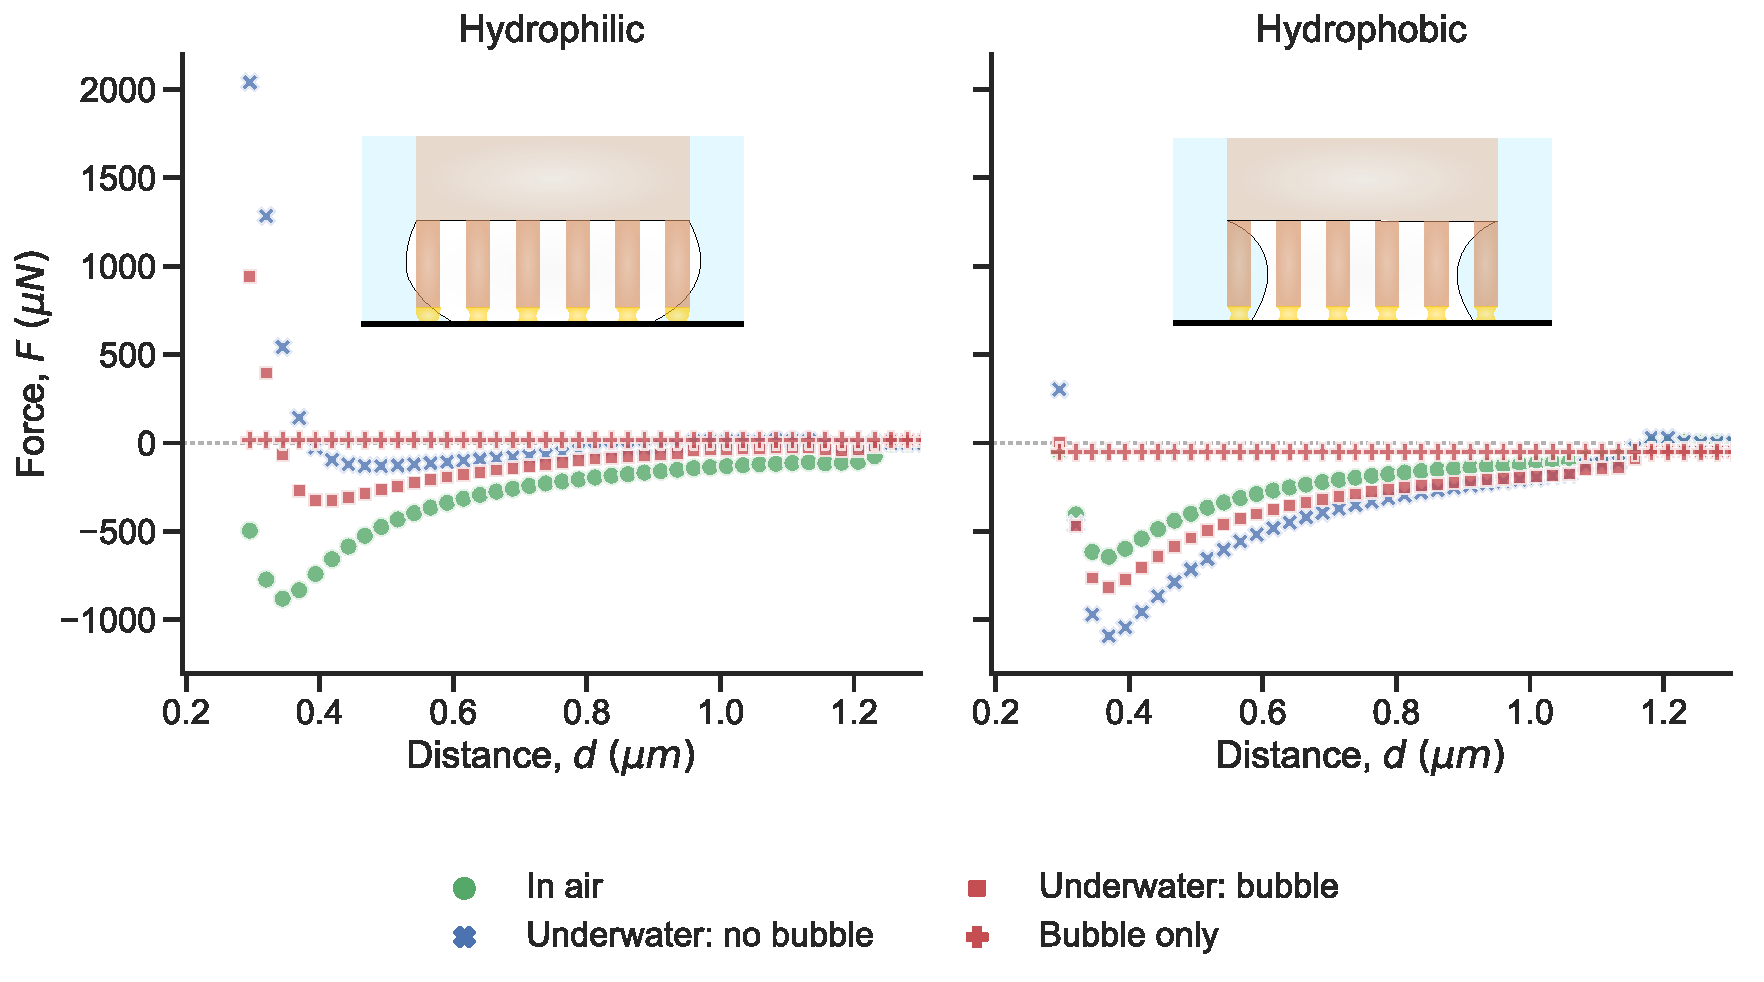
\includegraphics[width=6in]{Figure5-Model_effect_of_substrate}\caption{\label{fig:Effect-of-substrate}Theoretical force-distance curves
of a hairy pad on a hydrophilic and hydrophobic substrate in
air and underwater conditions. A negative force value represents attraction.
Normalised forces are calculated from the capillary bridge model,
with model parameters listed in Table \ref{tab:Model-parameters}.
The bubble's contribution to the net force for an \emph{underwater:
bubble} contact is denoted by plus symbols. Insets represent the \emph{underwater:
bubble }contact for each substrate.}
\end{figure*}

The observed trend in forces can be explained by how the tarsal adhesive
fluid wets the surface in each case. On a hydrophilic substrate, the
contact angle of the oily fluid is 6\textdegree , when surrounded
by air (Table \ref{tab:Model-parameters}) and 150\textdegree , when
surrounded by water (equation (\ref{eq:theta_fw})). This results
in the meniscus shape to have a net negative and slightly positive
curvatures, respectively, resulting in strong adhesion in air and
poor adhesion underwater. On a hydrophobic substrate however, the
contact angles of the fluid in air and water are 50\textdegree{} and
1\textdegree , respectively. In both cases, the contact angles are
low, resulting in strong adhesion in both media. Additionally, the
interfacial tension of the oily fluid underwater ($\gamma_{fw}$)
is twice that of in air ($\gamma_{fa}$). Thus, we see a higher capillary
adhesion for the \emph{underwater: no bubble} case when compared to
\emph{in air} (Figure \ref{fig:Oil-contact-images}). Note that the
contact area is fixed in all cases by keeping the area fraction and
$D_{p}/D_{h}$ constant. Thus the observed effects is not a result
of changing contact area, but rather on the nature of capillary forces.

\begin{figure}
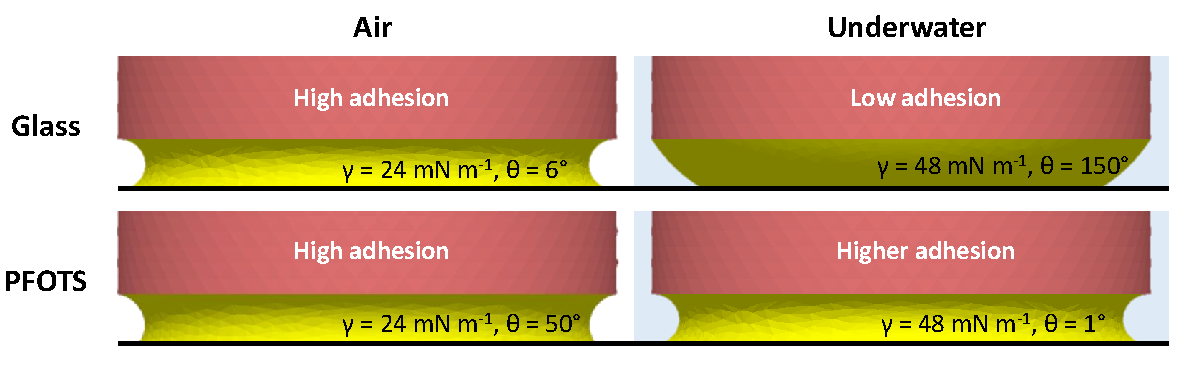
\includegraphics[width=3.5in]{Figure-8-contact_angle_schematic}\caption{\label{fig:Oil-contact-images}Simulation snapshots of oil capillary
meniscus in contact with untreated glass and PFOTS-coated glass in air and underwater conditions.
The corresponding interfacial tension, $\gamma$, and contact
angle, $\theta$, used to predict the ladybug's adhesion
are labelled for each case.}
\end{figure}

The net force in the \emph{underwater: bubble} case mainly depends
on the proportion of hairs inside and outside the bubble (equation
(\ref{eq:f_bubble})). For the given bubble volume, only part of the
hairs make contact with the surface inside the bubble for the hydrophilic case, while,
all the hairs contact the surface inside the bubble for the hydrophobic case.
Therefore, the force curve lies between \emph{in air} and \emph{underwater:
no bubble} cases for a hydrophilic substrate, and closely follows
the \emph{in air} case for a hydrophobic substrate.

We observed that the bubble itself does not contribute much to the net force
on either substrate (Figure \ref{fig:Effect-of-substrate}). Its contribution
even is slightly repulsive on the hydrophilic substrate due to the
positive curvature of the bubble, and slightly attractive on the hydrophobic
substrate due to its negative curvature. This small contribution is
manifested by the slightly higher adhesion for \emph{underwater: bubble}
relative to \emph{in air} for the hydrophobic substrate, since all
hairs are within the bubble in this case.

\subsection{Adhesion of a hairy pad: Effect of the air bubble volume}

The volume of the trapped air bubble can influence its capillary force contribution,
as well as change the relative proportion of hairs inside and outside
it. To investigate this, we varied the bubble volume, $\hat{V}_{b}$,
and compared the maximum adhesion force on both hydrophilic and hydrophobic
substrates (Figure \ref{fig:Effect-of-bubble}). The contribution
of the bubble to the net adhesion force is small regardless of its
volume, when compared to the whole pad. Further, opposite trends of
adhesion are seen on the two substrates with changing $\hat{V}_{b}$.

From the previous section, we know that on the hydrophilic substrate,
fluid bridges outside the bubble show poor adhesion due to the positive
curvature of their meniscus. Thus, decreasing $\hat{V}_{b}$ decreases
the adhesion force due to a larger proportion of tarsal hairs being outside
the bubble. In contrast, on the hydrophobic substrate, fluid bridges
outside the bubble showed higher capillary forces, due to its low contact
angle and high interfacial tension in water. Thus, adhesion force
increases for a hydrophobic substrate as the bubble size decreases. 

A smaller $\hat{V}_{b}$ resulted in increased, but small, attraction
by the bubble on both types of substrates. For larger values of $\hat{V}_{b}$
however, the force trend for the whole pad mostly follows that of
the bubble. This is because the bubble gets big enough to entrap all
the hairs inside it. Thus, the force contribution due to the fluid
bridges remain unchanged, and only the bubble's contribution drives
the slight variation in the pad's adhesion at high $\hat{V}_{b}$.
Once the bubble is small enough such that part of the fluid bridges
start making contact in water, the force trend changes, with a steep
decrease (increase) in adhesion force on hydrophilic (hydrophobic)
substrate as the volume decreases.

\begin{figure}
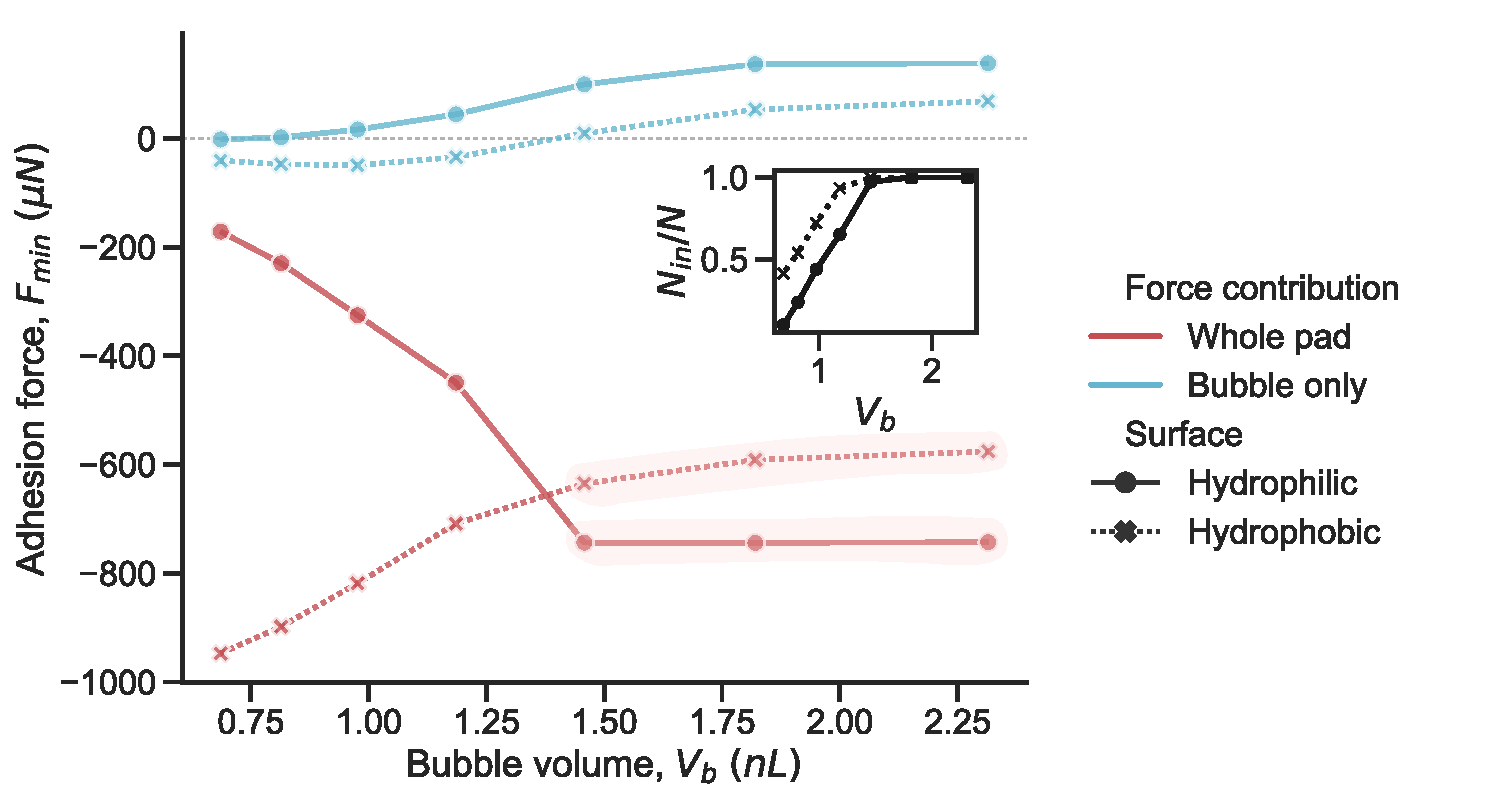
\includegraphics[width=3.5in]{Figure7-Model_effect_of_bubble_volume}\caption{\label{fig:Effect-of-bubble}Normalised adhesion force of a hairy
pad as a function of bubble volume, $\hat{V}_{b}$, for the
\emph{underwater: bubble} contact mode. Adhesion forces are calculated
from the minima of the respective force-distance curves. Negative
force value represents attraction. Pad to hair diameter ratio ($D_{p}/D_{h}$)
is kept fixed. Highlighted regions represent entrapment of all hairs
within the bubble.}
\end{figure}

%CHECK THIS!!%
\subsection{Adhesion of a hairy pad: Effect of the hair tip diameter}

\begin{figure}
%\centering
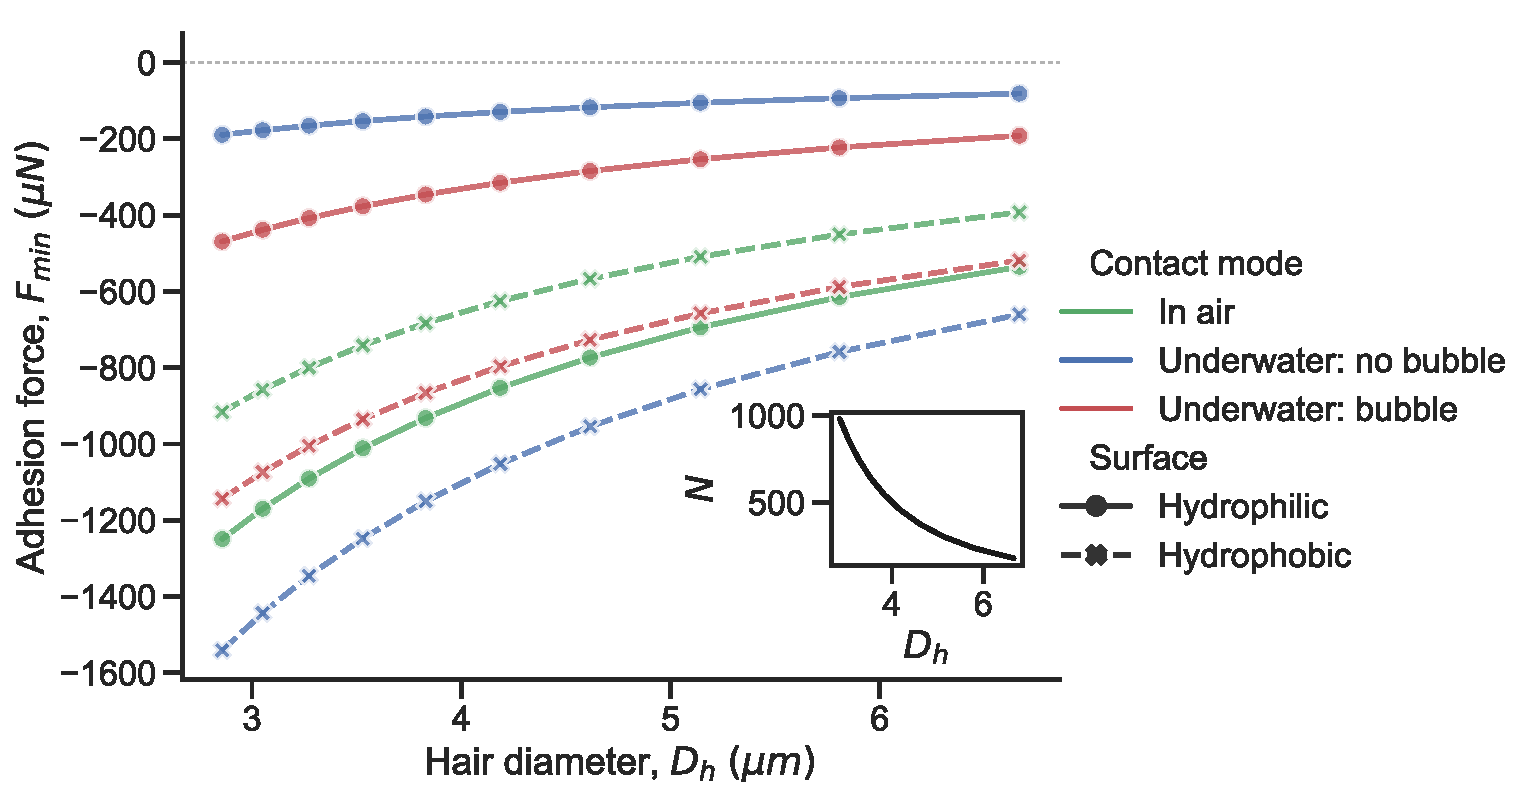
\includegraphics[width=3.5in]{Figure6-Model_effect_of_hair_size}
\caption{\label{fig:Effect-of-hair}Normalised adhesion force of a hairy pad on a hydrophilic and hydrophobic substrate as a function of
hair tip diameter, $D_{h}$. Volume of each fluid bridge, $V_{f}$, scales
relative to $D_{h}$ based on the parameter $\phi_{f}=2$. Adhesion
forces are calculated from the minima of the respective force-distance
curves, based on the capillary bridge model. A negative value represents
attraction. The air bubble's contribution to the net force for an \emph{underwater:
bubble} contact is denoted by plus symbols. Pad diameter and bubble
volume are kept fixed. All lengths are scaled relative to $D_{p}$.}
\end{figure}

The tarsal hairs on a ladybug's adhesive pad terminate in various shapes, such as ``discoidal''
or ``pointed''. We studied this geometric effect on adhesion by
changing the hair tip diameter, $D_{h}$ (Figure \ref{fig:Effect-of-hair}).
Here, the pad diameter, total hair contact area and bubble volume
are constant since $D_{p}$, $\alpha$ and $\hat{V}_{b}$ are kept
fixed. The tarsal adhesive fluid volume is again assumed to scale relative
to the hair diameter ($\phi_{f}=2$).

Adhesion force increases with decreasing $D_{h}$ for both hydrophilic
and hydrophobic substrates in all contact modes. This is consistent
with the ``contact splitting'' theory, which predicts higher adhesion
when the contact is split into many small contact points\citep{RN24}.
Reducing the hair diameter results in two competing effects: 1) capillary
force due to a single fluid bridge decreases due to its smaller size
and ``self-similar'' scaling assumption ($f\sim D_{h}$), which
decreases the net force, and 2) total number of fluid bridges increases
since the total hair contact area is assumed to be fixed ($N\sim1/D_{h}^{2}$),
which increases the net force. The second effect dominates, resulting
in a higher adhesion force as $D_{h}$ decreases. 

Similar to the trend in Figure \ref{fig:Effect-of-substrate}, contact
\emph{in air} shows the highest adhesion force on a hydrophilic substrate
for the given range of hair diameters, while on a hydrophobic substrate,
\emph{underwater: no bubble} shows highest adhesion. \emph{Underwater:
bubble} contact shows intermediate adhesion between \emph{in air}
and \emph{underwater: no bubble} contact modes.

The bubble's contribution gets repulsive as hair diameter decreases
for both substrates (Figure \ref{fig:Effect-of-hair}). Since the
aspect ratio $L/D_{h}$ is fixed (Table \ref{tab:Model-parameters}),
decreasing the hair diameter also decreases its length. Since the
bubble's volume is kept constant, it will then have a lesser space
available to occupy between the pad and the substrate. This results
in it bulging outwards near the pinned contact line on the top, causing
repulsion.

\section{Discussion}

Our experiments demonstrate that the ladybug beetle can attach underwater
to a hydrophobic substrate even without a bubble trapped around its
tarsal hairs. A previous study\citep{RN87} proposed that an air bubble
is necessary for underwater attachment in terrestrial beetles. This is, however,
only true for hydrophilic substrates, where a trapped air bubble can facilitate
underwater adhesion due to the hairs making contact in a de-wetted
environment. For a hydrophobic substrate, the adhesion is similar
regardless of whether the contact occurs in air or underwater conditions,
with or without a trapped bubble. Our theoretical calculations further
show that the bubble by itself has a negligible capillary contribution
to the net underwater adhesion of the pad. Direct force measurement
of a single similarly sized bubble making contact with a hydrophobic
substrate shows a maximum adhesion less than 50 \textmu N, which
further validates that the bubble's contribution is insignificant
(see supplementary section S4).

Predictions of the ladybug's adhesion from the capillary bridge model
agree with our experimental results (Figure \ref{fig:Effect-of-contact}).
In underwater conditions without a trapped air bubble, adhesion to a hydrophobic
substrate is significantly larger than to a hydrophilic substrate.
This is explained by the different interfacial tension of the oily tarsal secretion and its contact
angles with the substrates in air and underwater, which determines
the capillary adhesive force in each case (Figure \ref{fig:Oil-contact-images}).
However, the experiments do not show the predicted $\sim$ 2.6 times
increase in underwater adhesion relative to that in air on the hydrophobic
PFOTS-coated surface. This discrepancy could be due to our assumptions of
the oily fluid's interfacial properties. If we choose $\gamma_{fa}$=30
mN m\protect\textsuperscript{-1} and $\gamma_{fw}$=40 mN m\protect\textsuperscript{-1}, the corresponding increase in adhesion
will be $\sim$ 1.7, closer to our experimental value of $\sim$ 1.
The resulting change in $\theta_{fa}$ and $\theta_{fw}$ will further
decrease this number. Direct measurement of the fluid's interfacial
properties is thus essential to better predict the insect's adhesion,
and will be a subject of future studies. Further, due to surface inhomogeneities,
not all the hairs might be able to completely drain the interfacial
water layer, in order for the tarsal adhesive fluid to make direct contact
with the substrate. This can further reduce underwater adhesion, in
comparison to our theoretical predictions which assumes a perfect
contact of all hairs' terminals.

In the model, we assume that all the hairs detach simultaneously to
give a theoretical maximum achievable adhesion force. In our experiments,
however, not all hairs make a perfect contact with the substrate despite our 
best efforts to align the pad parallel to the surface. Furthermore, during detachment, 
the constrained pad typically peels off from its proximal to distal end rather
than detach simultaneously. Our model also assumes the hairs to be stiff and 
of similar geometry, unlike the male beetle's pad which has a distribution
of flat or pointed tipped soft hairs. Thus, it is not surprising that the
model overestimates the adhesion forces. However, when comparing the adhesion in air and underwater,
the effect of pad orientation, peeling, hair geometry or elasticity on adhesion should be similar for both cases, and thus, can be reasonably ignored. The model predictions are
in the same order of magnitude as experiments, and the qualitative
trend is consistent for both hydrophilic and hydrophobic substrates
in air and underwater.

Our study provides further validation that capillary forces govern the ladybug's adhesion and van der Waals contributions,
if any, must be negligible. Further, the capillary forces can even
enable ladybug attachment underwater depending on the substrate chemistry.
When underwater, without a trapped bubble, the pads adhere strongly
to a hydrophobic substrate, but poorly to a hydrophilic substrate,
even though the pad shows similarly strong adhesion to both substrates
in air. This effect can be explained by capillary forces and the wetting properties of the fluid. Our
preliminary chemical composition analysis of a beetle's tarsal secretions before and after immersing its leg underwater (unpublished data) suggests that the tarsal adhesive fluid do not get washed away when underwater. Therefore, the fluid should be able to form capillary bridges and help mediate adhesion even when underwater.

The presence of interfacial water was expected to cause adhesion loss during underwater contact. However, we see that, underwater adhesion is possible even for a hydrophilic surface without a trapped bubble (Figure \ref{fig:Effect-of-contact}). This suggests the possible role of interfacial water drainage dynamics on adhesion. The experimental adhesion values lie close the theoretical predictions, which suggests that the interfacial water is drained out within the time-scale of contact ($\sim$ 4 s). The tarsal fluid would then form capillary bridges in direct contact with the surface and enable adhesion. The details of this drainage mechanism during capillary mediated underwater adhesion would be interesting to look at in a future study.

To some extent, the findings could be extended to other animals relying on oily
secretions for adhesion. For example, ants are known to possess smooth adhesive pads which secrete a fluid containing oily substances \citep{RN201}.
It has been reported that some ants show similar adhesion on hydrophobic substrates under wet and dry conditions \citep{RN213},
similar to what we see in a ladybug. This observation can again be explained by a capillary model as before. Recent experiments on
geckos revealed that they can attach well to fluoropolymer substrates (such as PTFE)
underwater while they show little adhesion to the same substrate in
air\citep{RN199,RN15}. Geckos are thought to rely on van der Waals
forces via dry contact with the substrate \citep{RN202}, although
recent observations of phospholipid footprints left behind walking
geckos \citep{RN205} could change that picture. Since geckos adhere
poorly to PTFE (surface energy $\sim$ 20 mN m\protect\textsuperscript{-1}) one can
speculate that the phospholipid material has a higher surface energy,
and consequently makes a higher contact angle with PTFE in air. Let
us assume the phosopholipid substance to be a fluid similar to oil 
with $\gamma_{fa}$= 30 mN m\protect\textsuperscript{-1} and $\gamma_{fw}$= 42 mN m\protect\textsuperscript{-1} such that
its contact angle with PTFE is 80\textdegree . Equation \ref{eq:theta_fw}
then gives us an underwater contact angle of 70\textdegree{} for the
phospholipid fluid. Thus, on a PTFE surface, the capillary bridge
model can predict a higher adhesion underwater than in air due to
its lower contact angle and higher interfacial energy underwater.
Based on similar assumptions, we predict the net adhesion force for
the gecko on different substrates (Figure \ref{fig:Comparison-with-model}).
The adhesion force predictions are in good qualitative agreement with
the whole animal experimental shear force values reported for the
gecko, with the trend of higher adhesion in air than underwater for
glass, similar adhesion in air and underwater for PMMA/OTS-SAM and
lower adhesion in air than underwater for PTFE. We, thus, propose
that the underwater experiments performed on geckos \citep{RN199,RN15}
indicate a capillary contribution to gecko adhesion. Previous studies on gecko adhesion have attributed capillary effects to be a result of water monolayers adsorbed from ambient humid air onto the spatuale hair tips \citep{RN197, RN203, RN218}.
We however emphasize that capillary contribution in gecko adhesion could rather be a result of its setal phospholipid layer rather than water.
The previously reported influence of humidity on gecko adhesion \citep{RN197} could possibly be an effect of change in surface tension of the oily phospholipid layer at different humidity, which will in-turn influence the capillary adhesion force. We suggest performing single seta adhesion force tests similar to \citet{RN202}
using a hydrophilic and fluorinated probe in air and underwater conditions. 
If the fluorinated probe shows higher adhesion underwater than in air on a single seta, this
would confirm the role of capillary contributions due to an oil-like phospholipid layer to gecko adhesion. Further work is also necessary to validate if the phospholipid layer in geckos' toes indeed has fluid-like properties.

\begin{figure}
\centering
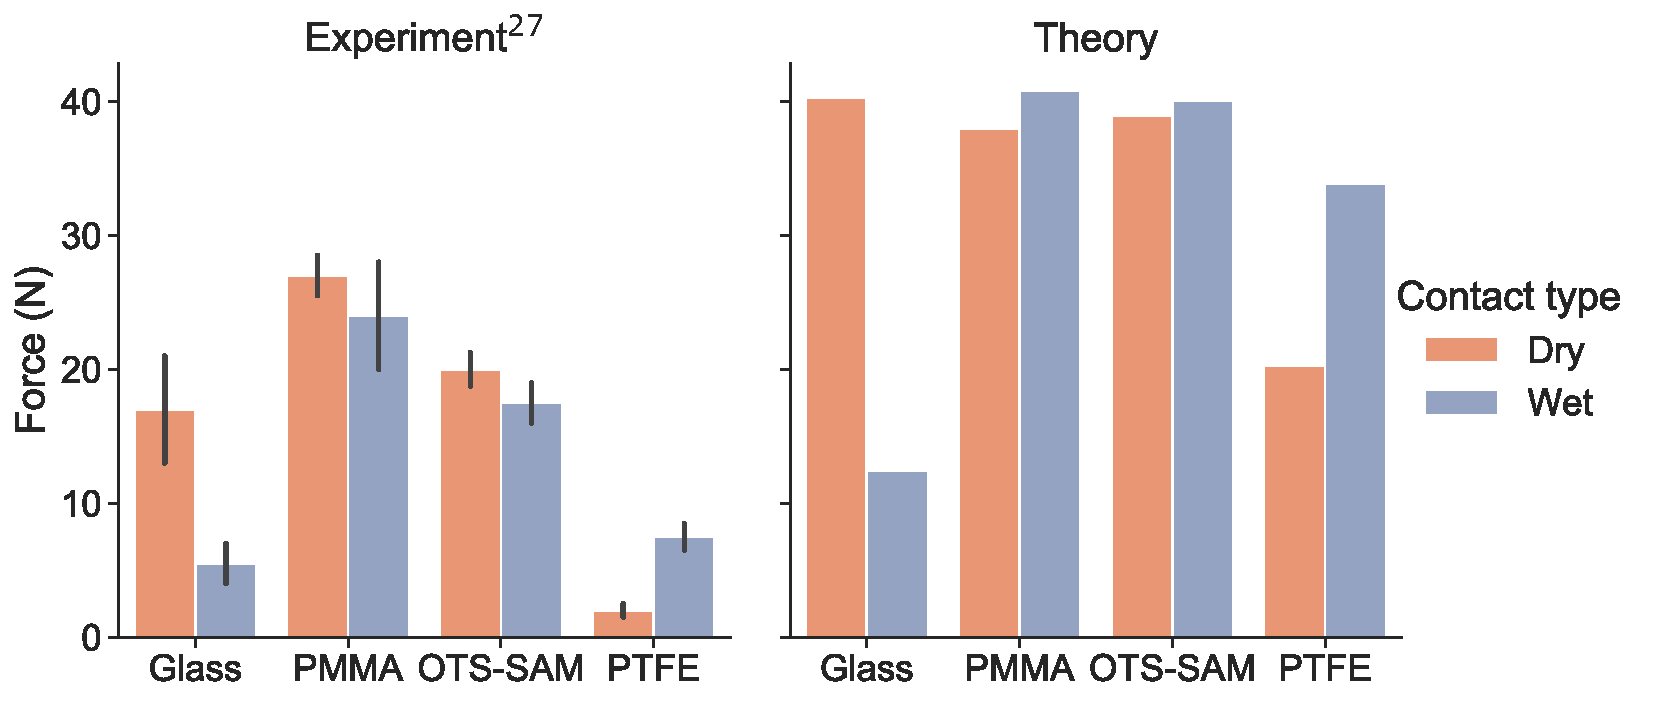
\includegraphics[width=3.5in]{Figure-9-Gecko_comparison}\caption{\label{fig:Comparison-with-model}Whole animal adhesion force of geckos
on various substrates. Experimental shear adhesion values are reproduced
from \citet{RN15}. Normal adhesion forces for each gecko
toe are theoretically estimated from the capillary bridge model, with
hair diameter = 400 nm, toe diameter = 4 mm, phospholipid fluid volume
= 4.19x10\protect\textsuperscript{-3} fL and 10\% hair coverage.
\textquotedblleft\emph{Underwater: no bubble}\textquotedblright{}
contact mode is assumed for the \textquotedblleft Wet\textquotedblright{}
case. Net adhesion force is calculated by assuming 5 toes on each
leg and 4 legs in total on a gecko. Interfacial tension of the phospholipid
layer (PL) in air and water are assumed to be 30 mN m\protect\textsuperscript{-1} and 42 mN m\protect\textsuperscript{-1}
respectively. PL contact angles with glass, PMMA, OTS-SAM and PTFE
are assumed to be 6\textdegree , 10\textdegree , 20\textdegree{} and
80\textdegree{} respectively. The corresponding water contact angles
are 50\textdegree , 85\textdegree , 94\textdegree{} and 97\textdegree{}
respectively, as reported in \citet{RN15}.}
\end{figure}

We have so far limited our analysis to only smooth substrates. Of course insects
have to cope with all kinds of surfaces including rough ones.
Previous studies \citep{RN136} have shown that substrate roughness
is a more dominant parameter than substrate chemistry in controlling
ladybug beetle traction force. Here, the length scale of surface roughness relative to the tarsal fluid thickness would be important in the formation of stable capillary bridges. Further, the presence of air plastron between the roughness asperities can influence the nature of contact when underwater. Future work will explore how roughness can impact
the net capillary force also in wet and submerged conditions. In our study, we have only considered normal adhesive forces, but insects like beetles in general rely on friction or shear forces during locomotion. Friction force usually correlates directly with the normal force, which is probably why previously reported shear adhesion forces of the dock beetle \citep{RN87} follow a similar qualitative trend as our normal adhesion force measurements on the ladybug beetle in both air and underwater conditions. However, the details of the interplay between friction and normal adhesion forces in animals is an open question and is beyond the scope of this paper. 

Our study can contribute to potential applications in the design of bio-inspired materials to achieve underwater adhesion
via capillary bridges. Introduced bubbles can possibly be used to control underwater
adhesion by changing the relative proportion of the arrays inside
and outside the bubble. A suitable choice of an adhesion-mediating fluid can be
made tailored to the substrate and environment of application to form capillary bridges with 
optimal adhesion performance in bio-inspired fibrillar adhesive systems.

\section{Conclusions}

Ladybug beetles rely primarily on their oily fluid secretion at the tarsal hair tips to adhere
to surfaces in both air and underwater conditions. The beetles can
attach underwater on a hydrophobic substrate even without a trapped
air bubble within its hairy pad, although it loses this ability on
a hydrophilic substrate. This is explained theoretically by the different
contact angle and interfacial tension of the secreted fluid in air
and underwater conditions. Further, the bubble itself has a negligible
capillary contribution to the total force. The trapped bubble can
promote adhesion only on a hydrophilic substrate by providing an air
medium to the adhesive fluid bridges inside it. Oil wettability, thus,
primarily controls the insect's adhesion in any given condition. 
Our study highlights how a fluid-mediated strategy can help achieve strong adhesion even underwater. A
similar argument also explains previously reported underwater adhesion force measurements
in geckos \citep{RN15}, which suggests the possibility of capillary
contributions to gecko adhesion mediated by an oil-like phospholipid layer. Future studies should characterise
the fluid secretion's interfacial properties with a particular substrate
to better understand the fundamental nature of an animal's adhesion.

%\section{Acknowledgements}

\ack{We are grateful to Prof. Dr. Eduard Arzt and Dr. Ren\' {e} Hensel (Leibniz Institute for New Materials, Saarbr\"{u}cken, Germany)  for fruitful discussions.} 

%\section{Competing interests}
\competing{The authors declare no competing or financial interests.}

%\section{Data availability}
%\data{Data are available from the Dryad digital repository.} %CHECK THIS%

%\section{Funding}
\funding{This work was supported by the \emph{Deutsche Forschungsgemeinschaft}
(Grant number: PI 1351/2-1) and the \emph{Max Planck Graduate Center} with the \emph{Johannes Gutenberg-Universit\"{a}t Mainz} (MPGC).} 

\bibliography{references}

\end{document}
